% Generated by Sphinx.
\def\sphinxdocclass{report}
\documentclass[letterpaper,10pt,english]{sphinxmanual}
\usepackage[utf8]{inputenc}
\DeclareUnicodeCharacter{00A0}{\nobreakspace}
\usepackage{cmap}
\usepackage[T1]{fontenc}
\usepackage{babel}
\usepackage{times}
\usepackage[Bjarne]{fncychap}
\usepackage{longtable}
\usepackage{sphinx}
\usepackage{multirow}


\title{AIMBAT Documentation}
\date{October 06, 2014}
\release{0.2.1}
\author{Lay Kuan Loh, Xiaoting Lou, \& Suzan van der Lee}
\newcommand{\sphinxlogo}{}
\renewcommand{\releasename}{Release}
\makeindex

\makeatletter
\def\PYG@reset{\let\PYG@it=\relax \let\PYG@bf=\relax%
    \let\PYG@ul=\relax \let\PYG@tc=\relax%
    \let\PYG@bc=\relax \let\PYG@ff=\relax}
\def\PYG@tok#1{\csname PYG@tok@#1\endcsname}
\def\PYG@toks#1+{\ifx\relax#1\empty\else%
    \PYG@tok{#1}\expandafter\PYG@toks\fi}
\def\PYG@do#1{\PYG@bc{\PYG@tc{\PYG@ul{%
    \PYG@it{\PYG@bf{\PYG@ff{#1}}}}}}}
\def\PYG#1#2{\PYG@reset\PYG@toks#1+\relax+\PYG@do{#2}}

\expandafter\def\csname PYG@tok@gd\endcsname{\def\PYG@tc##1{\textcolor[rgb]{0.63,0.00,0.00}{##1}}}
\expandafter\def\csname PYG@tok@gu\endcsname{\let\PYG@bf=\textbf\def\PYG@tc##1{\textcolor[rgb]{0.50,0.00,0.50}{##1}}}
\expandafter\def\csname PYG@tok@gt\endcsname{\def\PYG@tc##1{\textcolor[rgb]{0.00,0.27,0.87}{##1}}}
\expandafter\def\csname PYG@tok@gs\endcsname{\let\PYG@bf=\textbf}
\expandafter\def\csname PYG@tok@gr\endcsname{\def\PYG@tc##1{\textcolor[rgb]{1.00,0.00,0.00}{##1}}}
\expandafter\def\csname PYG@tok@cm\endcsname{\let\PYG@it=\textit\def\PYG@tc##1{\textcolor[rgb]{0.25,0.50,0.56}{##1}}}
\expandafter\def\csname PYG@tok@vg\endcsname{\def\PYG@tc##1{\textcolor[rgb]{0.73,0.38,0.84}{##1}}}
\expandafter\def\csname PYG@tok@m\endcsname{\def\PYG@tc##1{\textcolor[rgb]{0.13,0.50,0.31}{##1}}}
\expandafter\def\csname PYG@tok@mh\endcsname{\def\PYG@tc##1{\textcolor[rgb]{0.13,0.50,0.31}{##1}}}
\expandafter\def\csname PYG@tok@cs\endcsname{\def\PYG@tc##1{\textcolor[rgb]{0.25,0.50,0.56}{##1}}\def\PYG@bc##1{\setlength{\fboxsep}{0pt}\colorbox[rgb]{1.00,0.94,0.94}{\strut ##1}}}
\expandafter\def\csname PYG@tok@ge\endcsname{\let\PYG@it=\textit}
\expandafter\def\csname PYG@tok@vc\endcsname{\def\PYG@tc##1{\textcolor[rgb]{0.73,0.38,0.84}{##1}}}
\expandafter\def\csname PYG@tok@il\endcsname{\def\PYG@tc##1{\textcolor[rgb]{0.13,0.50,0.31}{##1}}}
\expandafter\def\csname PYG@tok@go\endcsname{\def\PYG@tc##1{\textcolor[rgb]{0.20,0.20,0.20}{##1}}}
\expandafter\def\csname PYG@tok@cp\endcsname{\def\PYG@tc##1{\textcolor[rgb]{0.00,0.44,0.13}{##1}}}
\expandafter\def\csname PYG@tok@gi\endcsname{\def\PYG@tc##1{\textcolor[rgb]{0.00,0.63,0.00}{##1}}}
\expandafter\def\csname PYG@tok@gh\endcsname{\let\PYG@bf=\textbf\def\PYG@tc##1{\textcolor[rgb]{0.00,0.00,0.50}{##1}}}
\expandafter\def\csname PYG@tok@ni\endcsname{\let\PYG@bf=\textbf\def\PYG@tc##1{\textcolor[rgb]{0.84,0.33,0.22}{##1}}}
\expandafter\def\csname PYG@tok@nl\endcsname{\let\PYG@bf=\textbf\def\PYG@tc##1{\textcolor[rgb]{0.00,0.13,0.44}{##1}}}
\expandafter\def\csname PYG@tok@nn\endcsname{\let\PYG@bf=\textbf\def\PYG@tc##1{\textcolor[rgb]{0.05,0.52,0.71}{##1}}}
\expandafter\def\csname PYG@tok@no\endcsname{\def\PYG@tc##1{\textcolor[rgb]{0.38,0.68,0.84}{##1}}}
\expandafter\def\csname PYG@tok@na\endcsname{\def\PYG@tc##1{\textcolor[rgb]{0.25,0.44,0.63}{##1}}}
\expandafter\def\csname PYG@tok@nb\endcsname{\def\PYG@tc##1{\textcolor[rgb]{0.00,0.44,0.13}{##1}}}
\expandafter\def\csname PYG@tok@nc\endcsname{\let\PYG@bf=\textbf\def\PYG@tc##1{\textcolor[rgb]{0.05,0.52,0.71}{##1}}}
\expandafter\def\csname PYG@tok@nd\endcsname{\let\PYG@bf=\textbf\def\PYG@tc##1{\textcolor[rgb]{0.33,0.33,0.33}{##1}}}
\expandafter\def\csname PYG@tok@ne\endcsname{\def\PYG@tc##1{\textcolor[rgb]{0.00,0.44,0.13}{##1}}}
\expandafter\def\csname PYG@tok@nf\endcsname{\def\PYG@tc##1{\textcolor[rgb]{0.02,0.16,0.49}{##1}}}
\expandafter\def\csname PYG@tok@si\endcsname{\let\PYG@it=\textit\def\PYG@tc##1{\textcolor[rgb]{0.44,0.63,0.82}{##1}}}
\expandafter\def\csname PYG@tok@s2\endcsname{\def\PYG@tc##1{\textcolor[rgb]{0.25,0.44,0.63}{##1}}}
\expandafter\def\csname PYG@tok@vi\endcsname{\def\PYG@tc##1{\textcolor[rgb]{0.73,0.38,0.84}{##1}}}
\expandafter\def\csname PYG@tok@nt\endcsname{\let\PYG@bf=\textbf\def\PYG@tc##1{\textcolor[rgb]{0.02,0.16,0.45}{##1}}}
\expandafter\def\csname PYG@tok@nv\endcsname{\def\PYG@tc##1{\textcolor[rgb]{0.73,0.38,0.84}{##1}}}
\expandafter\def\csname PYG@tok@s1\endcsname{\def\PYG@tc##1{\textcolor[rgb]{0.25,0.44,0.63}{##1}}}
\expandafter\def\csname PYG@tok@gp\endcsname{\let\PYG@bf=\textbf\def\PYG@tc##1{\textcolor[rgb]{0.78,0.36,0.04}{##1}}}
\expandafter\def\csname PYG@tok@sh\endcsname{\def\PYG@tc##1{\textcolor[rgb]{0.25,0.44,0.63}{##1}}}
\expandafter\def\csname PYG@tok@ow\endcsname{\let\PYG@bf=\textbf\def\PYG@tc##1{\textcolor[rgb]{0.00,0.44,0.13}{##1}}}
\expandafter\def\csname PYG@tok@sx\endcsname{\def\PYG@tc##1{\textcolor[rgb]{0.78,0.36,0.04}{##1}}}
\expandafter\def\csname PYG@tok@bp\endcsname{\def\PYG@tc##1{\textcolor[rgb]{0.00,0.44,0.13}{##1}}}
\expandafter\def\csname PYG@tok@c1\endcsname{\let\PYG@it=\textit\def\PYG@tc##1{\textcolor[rgb]{0.25,0.50,0.56}{##1}}}
\expandafter\def\csname PYG@tok@kc\endcsname{\let\PYG@bf=\textbf\def\PYG@tc##1{\textcolor[rgb]{0.00,0.44,0.13}{##1}}}
\expandafter\def\csname PYG@tok@c\endcsname{\let\PYG@it=\textit\def\PYG@tc##1{\textcolor[rgb]{0.25,0.50,0.56}{##1}}}
\expandafter\def\csname PYG@tok@mf\endcsname{\def\PYG@tc##1{\textcolor[rgb]{0.13,0.50,0.31}{##1}}}
\expandafter\def\csname PYG@tok@err\endcsname{\def\PYG@bc##1{\setlength{\fboxsep}{0pt}\fcolorbox[rgb]{1.00,0.00,0.00}{1,1,1}{\strut ##1}}}
\expandafter\def\csname PYG@tok@kd\endcsname{\let\PYG@bf=\textbf\def\PYG@tc##1{\textcolor[rgb]{0.00,0.44,0.13}{##1}}}
\expandafter\def\csname PYG@tok@ss\endcsname{\def\PYG@tc##1{\textcolor[rgb]{0.32,0.47,0.09}{##1}}}
\expandafter\def\csname PYG@tok@sr\endcsname{\def\PYG@tc##1{\textcolor[rgb]{0.14,0.33,0.53}{##1}}}
\expandafter\def\csname PYG@tok@mo\endcsname{\def\PYG@tc##1{\textcolor[rgb]{0.13,0.50,0.31}{##1}}}
\expandafter\def\csname PYG@tok@mi\endcsname{\def\PYG@tc##1{\textcolor[rgb]{0.13,0.50,0.31}{##1}}}
\expandafter\def\csname PYG@tok@kn\endcsname{\let\PYG@bf=\textbf\def\PYG@tc##1{\textcolor[rgb]{0.00,0.44,0.13}{##1}}}
\expandafter\def\csname PYG@tok@o\endcsname{\def\PYG@tc##1{\textcolor[rgb]{0.40,0.40,0.40}{##1}}}
\expandafter\def\csname PYG@tok@kr\endcsname{\let\PYG@bf=\textbf\def\PYG@tc##1{\textcolor[rgb]{0.00,0.44,0.13}{##1}}}
\expandafter\def\csname PYG@tok@s\endcsname{\def\PYG@tc##1{\textcolor[rgb]{0.25,0.44,0.63}{##1}}}
\expandafter\def\csname PYG@tok@kp\endcsname{\def\PYG@tc##1{\textcolor[rgb]{0.00,0.44,0.13}{##1}}}
\expandafter\def\csname PYG@tok@w\endcsname{\def\PYG@tc##1{\textcolor[rgb]{0.73,0.73,0.73}{##1}}}
\expandafter\def\csname PYG@tok@kt\endcsname{\def\PYG@tc##1{\textcolor[rgb]{0.56,0.13,0.00}{##1}}}
\expandafter\def\csname PYG@tok@sc\endcsname{\def\PYG@tc##1{\textcolor[rgb]{0.25,0.44,0.63}{##1}}}
\expandafter\def\csname PYG@tok@sb\endcsname{\def\PYG@tc##1{\textcolor[rgb]{0.25,0.44,0.63}{##1}}}
\expandafter\def\csname PYG@tok@k\endcsname{\let\PYG@bf=\textbf\def\PYG@tc##1{\textcolor[rgb]{0.00,0.44,0.13}{##1}}}
\expandafter\def\csname PYG@tok@se\endcsname{\let\PYG@bf=\textbf\def\PYG@tc##1{\textcolor[rgb]{0.25,0.44,0.63}{##1}}}
\expandafter\def\csname PYG@tok@sd\endcsname{\let\PYG@it=\textit\def\PYG@tc##1{\textcolor[rgb]{0.25,0.44,0.63}{##1}}}

\def\PYGZbs{\char`\\}
\def\PYGZus{\char`\_}
\def\PYGZob{\char`\{}
\def\PYGZcb{\char`\}}
\def\PYGZca{\char`\^}
\def\PYGZam{\char`\&}
\def\PYGZlt{\char`\<}
\def\PYGZgt{\char`\>}
\def\PYGZsh{\char`\#}
\def\PYGZpc{\char`\%}
\def\PYGZdl{\char`\$}
\def\PYGZhy{\char`\-}
\def\PYGZsq{\char`\'}
\def\PYGZdq{\char`\"}
\def\PYGZti{\char`\~}
% for compatibility with earlier versions
\def\PYGZat{@}
\def\PYGZlb{[}
\def\PYGZrb{]}
\makeatother

\renewcommand\PYGZsq{\textquotesingle}

\begin{document}

\maketitle
\tableofcontents
\phantomsection\label{index::doc}


Contents:


\includegraphics{NU_Logo_purple.jpg}


\chapter{Introduction}
\label{docfiles/introduction:introduction}\label{docfiles/introduction:welcome-to-aimbat-s-documentation}\label{docfiles/introduction::doc}

\section{About AIMBAT}
\label{docfiles/introduction:about-aimbat}
AIMBAT (Automated and Interactive Measurement of Body wave Arrival Times) is an open-source software package for efficiently measuring teleseismic body wave arrival times for large seismic arrays {\hyperref[docfiles/citations:louvanderlee2013]{{[}LouVanDerLee2013{]}}}. It is based on a widely used method called MCCC (Multi-Channel Cross-Correlation) {\hyperref[docfiles/citations:vandecarcrosson1990]{{[}VanDecarCrosson1990{]}}}. The package is automated in the sense of initially aligning seismograms for MCCC which is achieved by an ICCS (Iterative Cross Correlation and Stack) algorithm. Meanwhile, a GUI (graphical user interface) is built to perform seismogram quality control interactively. Therefore, user processing time is reduced while valuable input from a user's expertise is retained. As a byproduct, SAC {\hyperref[docfiles/citations:goldsteindodge2003]{{[}GoldsteinDodge2003{]}}} plotting and phase picking functionalities are replicated and enhanced.

Modules and scripts included in the AIMBAT package were developed using \href{http://www.python.org/}{Python programming language} and its open-source modules on the Mac OS X platform since 2009. The original MCCC {\hyperref[docfiles/citations:vandecarcrosson1990]{{[}VanDecarCrosson1990{]}}} code was transcribed into Python. The GUI of AIMBAT was inspired and initiated at the \href{http://www.iris.edu/hq/es\_course/content/2009.html}{2009 EarthScope USArray Data Processing and Analysis Short Course}. AIMBAT runs on Mac OS X, Linux/Unix and Windows thanks to the platform-independent feature of Python. It has been tested on Mac OS 10.6.8 and 10.7 and Fedora 16.

The AIMBAT software package is distributed under the \href{http://www.gnu.org/licenses/gpl.html}{GNU General Public License Version 3 (GPLv3)} as published by the Free Software Foundation.


\section{Associated Documents}
\label{docfiles/introduction:associated-documents}\begin{itemize}
\item {} 
\code{Seismological Research Letters Paper}

\item {} 
\code{PDF Version of Manual}. Automatically generated from these online docs, please excuse minor issues that may arise from automated conversion.

\end{itemize}


\section{Authors' Contacts}
\label{docfiles/introduction:authors-contacts}\label{docfiles/introduction:id5}\begin{itemize}
\item {} 
\href{http://lkloh2410.wordpress.com/}{Lay Kuan Loh}

Email: lloh at ece.cmu.edu

\item {} 
\href{http://www.earth.northwestern.edu/~xlou/Welcome.html}{Xiaoting Lou}

Email: xlou at u.northwestern.edu

\item {} 
\href{http://www.earth.northwestern.edu/research/suzan/}{Suzan van der Lee}

Email: suzan at earth.northwestern.edu

\end{itemize}


\chapter{Installing Dependencies}
\label{docfiles/install_dependencies:installing-dependencies}\label{docfiles/install_dependencies::doc}
AIMBAT is build on top of \href{https://www.python.org/}{standard Python}, and uses several extra Python libraries as well. This page guides the user through checking if the required libraries are already install on the computer they want to install AIMBAT in, and how to get them if not.

To install AIMBAT, you will need sudo/root privileges for the computer you are installing it on.


\section{Getting your operating system}
\label{docfiles/install_dependencies:getting-your-operating-system}
We assume that most users of AIMBAT will be using Macs. If our assumptions are wrong, please {\hyperref[docfiles/introduction:authors-contacts]{\emph{contact the authors}}}, and if there is sufficient interest we will test and write documentation for installations on other operating systems as well.

On a mac, to find the version of your operating system, first click on the apple icon on the top bar of your desktop, go to \code{System Preferences}, and click on \code{Startup Disk}. The operating system version should then be displayed.

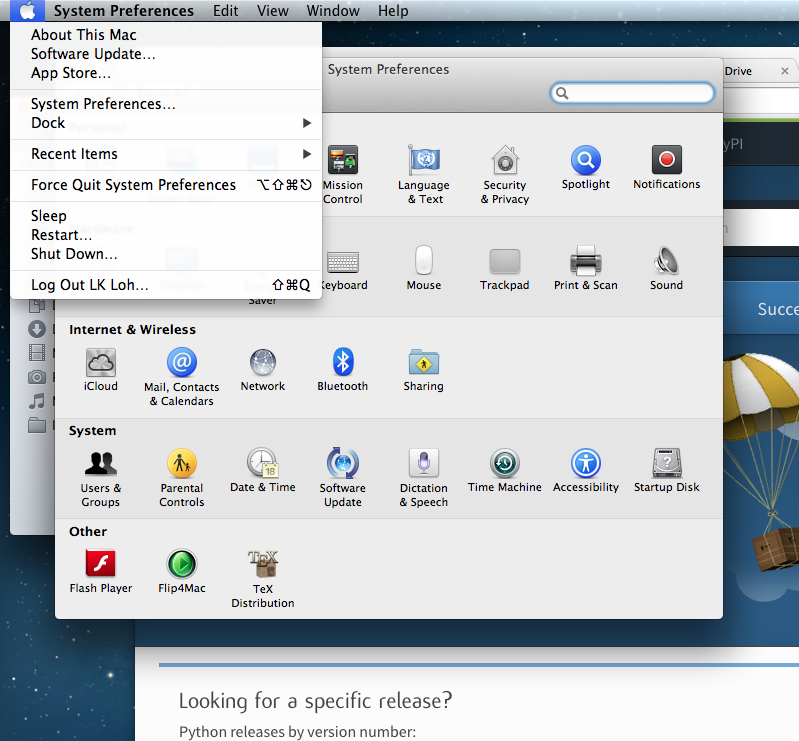
\includegraphics{system_preferences.png}


\section{Which Version of AIMBAT?}
\label{docfiles/install_dependencies:which-version-of-aimbat}
As AIMBAT uses several python dependencies, some of which are not critical to the primary function of picking travel-wave arrival times, \href{https://github.com/pysmo/aimbat-stable}{aimbat-stable} is recommended for users who do want to install \href{https://github.com/obspy/obspy/wiki}{obspy} and \href{http://matplotlib.org/basemap/}{basemap}, as they can sometimes be tricky to install.

The \href{https://github.com/pysmo/aimbat}{enhanced version} also allows for plotting the station locations on a map, converting pickle files into sac files, and running unit tests, which are relevant only to developers.


\section{Github}
\label{docfiles/install_dependencies:github}
\emph{Optional but recommended}.

The \href{https://github.com/pysmo}{latest version of AIMBAT} will be on \href{https://github.com/}{Github}, so it would be good to get \href{https://github.com/}{GitHub} on your computer. This is not strictly necessary, as you could also download it as a zipfile from the \href{http://www.earth.northwestern.edu/~xlou/aimbat.html}{AIMBAT website}.

To check if you already have \href{https://github.com/}{Github} installed, open the terminal and type:

\begin{Verbatim}[commandchars=\\\{\}]
\PYG{n}{git} \PYG{o}{\PYGZhy{}}\PYG{o}{\PYGZhy{}}\PYG{n}{version}
\end{Verbatim}

If GitHub is installed, the terminal should output a line describing the version number of GitHub installed on the computer, such as:

\begin{Verbatim}[commandchars=\\\{\}]
git version 1.8.5.2 (Apple Git\PYGZhy{}48)
\end{Verbatim}

If GitHub is not installed, the terminal will respond by telling you that it is not possible to issue this command:

\begin{Verbatim}[commandchars=\\\{\}]
\PYGZhy{}bash: git: command not found
\end{Verbatim}

To install GitHub, download the package installer \href{http://git-scm.com/download/mac}{here}. This would allow only command line usage of Git, so if you want to use a GUI, we recommend \href{https://mac.github.com/}{Git for Mac}.


\section{MacPorts}
\label{docfiles/install_dependencies:macports}
\href{http://www.macports.org/}{MacPorts} is a package management system that will be needed to install some python libraries.

To check if MacPorts is installed already, in the terminal, type:

\begin{Verbatim}[commandchars=\\\{\}]
port version
\end{Verbatim}

If MacPorts is installed, you should see the terminal output the version number, for instance:

\begin{Verbatim}[commandchars=\\\{\}]
Version: 2.3.0
\end{Verbatim}

If MacPorts is not installed, you should see the terminal complain that \code{port} is not a valid command:

\begin{Verbatim}[commandchars=\\\{\}]
\PYGZhy{}bash: port: command not found
\end{Verbatim}

To get MacPorts, download the package installer \href{http://www.macports.org/install.php}{here} and follow the instructions to install it. Be sure to get the right version of MacPorts for your operating system.


\section{Python and its Dependencies}
\label{docfiles/install_dependencies:python-and-its-dependencies}
AIMBAT requires python 2.7 and above to run. Note that Python is usually installed by default on Mac computers.

AIMBAT requires the following packages to run:
\#. \href{http://www.numpy.org/}{Numpy}: Used for manipulating numbers and datasets
\#. \href{http://www.scipy.org/}{Scipy}: Used for data processing
\#. \href{http://matplotlib.org/}{Matplotlib}: Used for the majority of the plots in AIMBAT and the GUI
\#. \href{http://matplotlib.org/basemap/}{Basemap}: Used for plotting world maps


\subsection{Checking if Python is installed}
\label{docfiles/install_dependencies:checking-if-python-is-installed}
Open the terminal and type:

\begin{Verbatim}[commandchars=\\\{\}]
\PYG{n}{python} \PYG{o}{\PYGZhy{}}\PYG{o}{\PYGZhy{}}\PYG{n}{version}
\end{Verbatim}

If Python is installed, the terminal will output the version number installed, for example:

\begin{Verbatim}[commandchars=\\\{\}]
Python 2.7.8
\end{Verbatim}

If Python is not installed, the terminal will output:

\begin{Verbatim}[commandchars=\\\{\}]
\PYGZhy{}bash: python: command not found
\end{Verbatim}


\subsection{If Python is not installed}
\label{docfiles/install_dependencies:if-python-is-not-installed}
Inside the terminal, once python is installed, type these commands in using sudo mode. Note you will need to enter your admin password.:

\begin{Verbatim}[commandchars=\\\{\}]
sudo port install py27
sudo port install py27\PYGZhy{}numpy
sudo port install py27\PYGZhy{}scipy
sudo port install py27\PYGZhy{}matplotlib
sudo port install py27\PYGZhy{}matplotlib\PYGZhy{}basemap
sudo port install py27\PYGZhy{}ipython
sudo port install python\PYGZus{}select
\end{Verbatim}

Installing the last two packages is optional. \code{ipython} is an enhanced interactive python shell. \code{python\_select} is used to select default Python version by the following command:

\begin{Verbatim}[commandchars=\\\{\}]
port select \PYGZhy{}\PYGZhy{}set python python27
\end{Verbatim}


\subsection{If Python is already installed}
\label{docfiles/install_dependencies:if-python-is-already-installed}
If Python is already installed, first check if you have the four required dependencies. Open up the Python console by typing:

\begin{Verbatim}[commandchars=\\\{\}]
\PYG{n}{python}
\end{Verbatim}

in the terminal. You should see something like this as output:

\begin{Verbatim}[commandchars=\\\{\}]
Python 2.7.8 (default, Oct  3 2014, 02:34:26)
[GCC 4.2.1 Compatible Apple LLVM 5.1 (clang\PYGZhy{}503.0.40)] on darwin
Type \PYGZdq{}help\PYGZdq{}, \PYGZdq{}copyright\PYGZdq{}, \PYGZdq{}credits\PYGZdq{} or \PYGZdq{}license\PYGZdq{} for more information.
\PYGZgt{}\PYGZgt{}\PYGZgt{}
\end{Verbatim}

Now, check if the packages have been installed properly by typing the following in:

\begin{Verbatim}[commandchars=\\\{\}]
\PYG{k+kn}{import} \PYG{n+nn}{numpy}
\PYG{k+kn}{import} \PYG{n+nn}{scipy}
\PYG{k+kn}{import} \PYG{n+nn}{matplotlib}
\PYG{k+kn}{from} \PYG{n+nn}{mpl\PYGZus{}toolkits.basemap} \PYG{k+kn}{import} \PYG{n}{Basemap}
\end{Verbatim}

If any of the packages are missing (e.g. scipy not installed), the python console will output an error, for instance:

\begin{Verbatim}[commandchars=\\\{\}]
Traceback (most recent call last):
File \PYGZdq{}\PYGZlt{}stdin\PYGZgt{}\PYGZdq{}, line 1, in \PYGZlt{}module\PYGZgt{}
ImportError: No module named scipy
\end{Verbatim}

Otherwise, the python console will simply show that it is ready for the next command.

If any of the packages are missing, you can choose to install it by whatever means you are most comfortable with. We provide one possible way to do so using MacPorts below. In the terminal, type:

\begin{Verbatim}[commandchars=\\\{\}]
sudo port install py27
\end{Verbatim}

to get the python version installed in \emph{opt/local/bin} where MacPort installs everything to. Select to use this version of Python by typing:

\begin{Verbatim}[commandchars=\\\{\}]
sudo port install python\PYGZus{}select
\end{Verbatim}

Now, install the missing packages by doing:

\begin{Verbatim}[commandchars=\\\{\}]
sudo port install py27\PYGZhy{}numpy
sudo port install py27\PYGZhy{}scipy
sudo port install py27\PYGZhy{}matplotlib
sudo port install py27\PYGZhy{}matplotlib\PYGZhy{}basemap
\end{Verbatim}


\section{Installing Basemap without MacPorts}
\label{docfiles/install_dependencies:installing-basemap-without-macports}
If you have already installed Basemap, which means that:

\begin{Verbatim}[commandchars=\\\{\}]
\PYG{k+kn}{from} \PYG{n+nn}{mpl\PYGZus{}toolkits.basemap} \PYG{k+kn}{import} \PYG{n}{Basemap}
\end{Verbatim}

comes out without an error in the Python console, you can skip this section. This is for users who do not want to use the MacPorts version of Python which has been installed to \emph{/opt/local/bin}. We anticipate that users who installed the official version of Python from the \href{https://www.python.org/}{Python website} may possible find this section useful.

Disclaimer: Lifted from content written by \href{http://blog.bluedackers.com/2012/11/13/installing-basemap-on-mac-os-x-mountain-lion/}{this guy} with some tweaks.

Enthough Python should get you most of the dependencies needed. You do need to get \href{http://trac.osgeo.org/geos/}{Geos} though. The best way to get it is \href{http://matthewcarriere.com/2013/08/05/how-to-install-and-use-homebrew/}{install Homebrew}, and then install \code{gdal}, a package that has \code{Geos} as a dependency. To get \code{gdal}, do:

\begin{Verbatim}[commandchars=\\\{\}]
brew install gdal
\end{Verbatim}

Now install Basemap. Download it \href{https://pypi.python.org/pypi/basemap}{here}. Unzip the package and cd into the unzipped package. To install basemap, do:

\begin{Verbatim}[commandchars=\\\{\}]
sudo python setup.py build
sudo python setup.py install
\end{Verbatim}

To check it worked, at the terminal, do:

\begin{Verbatim}[commandchars=\\\{\}]
\PYG{n}{python}
\end{Verbatim}

and then:

\begin{Verbatim}[commandchars=\\\{\}]
\PYG{k+kn}{from} \PYG{n+nn}{mpl\PYGZus{}toolkits.basemap} \PYG{k+kn}{import} \PYG{n}{Basemap}
\end{Verbatim}


\section{Possible Issues}
\label{docfiles/install_dependencies:possible-issues}
Here some common problems and possible resolutions. If your problem is not listed here, or you have a suggestion, please {\hyperref[docfiles/introduction:authors-contacts]{\emph{contact the authors}}}.


\subsection{Macports}
\label{docfiles/install_dependencies:id8}
You may run into problems with AIMBAT if your \href{http://www.macports.org/}{Macport} version is not compatible with your operating system version. For example, if you used Macports for OS X 10.8 to install AIMBAT, then upgraded your operating system or OS X 10.9, you may find that AIMBAT no longer works properly. You will need to upgrade Macports to fix this error.

Do not uninstall MacPorts unless you know what you are doing, uninstalling MacPorts may get rid of other programs you installed using MacPorts. However, if you are sure you want to do so, see \href{https://guide.macports.org/chunked/installing.macports.uninstalling.html}{here} for instructions.


\subsection{Installing Python with Pip}
\label{docfiles/install_dependencies:installing-python-with-pip}
Be careful with the operating system. For OS X 10.9 and above, Python 2.7 is not fully compatible and there may be problems installing python with Pip. Best to use Enthought Canopy or Python 3 with OS X 10.9.


\subsection{Setting the Python Path to the scripts}
\label{docfiles/install_dependencies:setting-the-python-path-to-the-scripts}
You are asked to add the path to the AIMBAT scripts in your file. To do that, you add them to the \code{.bashrc} file. There are other files you could add it to that work as well, such as the \code{.profile} or \code{.bash\_profile} files. You can see the files by opening the terminal and doing \code{ls -a} to see all the hidden files, and open then by doing \code{vi .bashrc} in vim, for instance.
To ensure you can open a script, you need to add:

\begin{Verbatim}[commandchars=\\\{\}]
export PATH=\PYGZdl{}PATH:\PYGZlt{}path\PYGZhy{}to\PYGZhy{}folder\PYGZhy{}with\PYGZhy{}scripts\PYGZgt{}
export PYTHONPATH=\PYGZdl{}PYTHONPATH:\PYGZlt{}path\PYGZhy{}to\PYGZhy{}folder\PYGZhy{}with\PYGZhy{}scripts\PYGZgt{}
\end{Verbatim}

to the \code{.bashrc} file. We recommend adding the paths to the \code{.bashrc} file.


\subsection{Terminal Commands stop working}
\label{docfiles/install_dependencies:terminal-commands-stop-working}
If ever the terminal commands such as ls stop working in the terminal, it could be that something went wrong with a path in the \code{.bashrc} or \code{.profile} files. If that happens you may not be able to open them in vim as that command would have stopped working as well. Instead, in the terminal, you do:

\begin{Verbatim}[commandchars=\\\{\}]
PATH=/bin:\PYGZdl{}\PYGZob{}PATH\PYGZcb{}
PATH=/usr/bin:\PYGZdl{}\PYGZob{}PATH\PYGZcb{}
\end{Verbatim}

And that should allow the commands to start working again. Figure out what you did wrong and remove that command.


\subsection{Installing Enthought Canopy}
\label{docfiles/install_dependencies:installing-enthought-canopy}
Occasionally, Enthought Canopy may not open the default setup environment after you downloaded and tried to install it. If this happens, open the Canopy package, go to ``Preferences'', and select Canopy as your default environment.

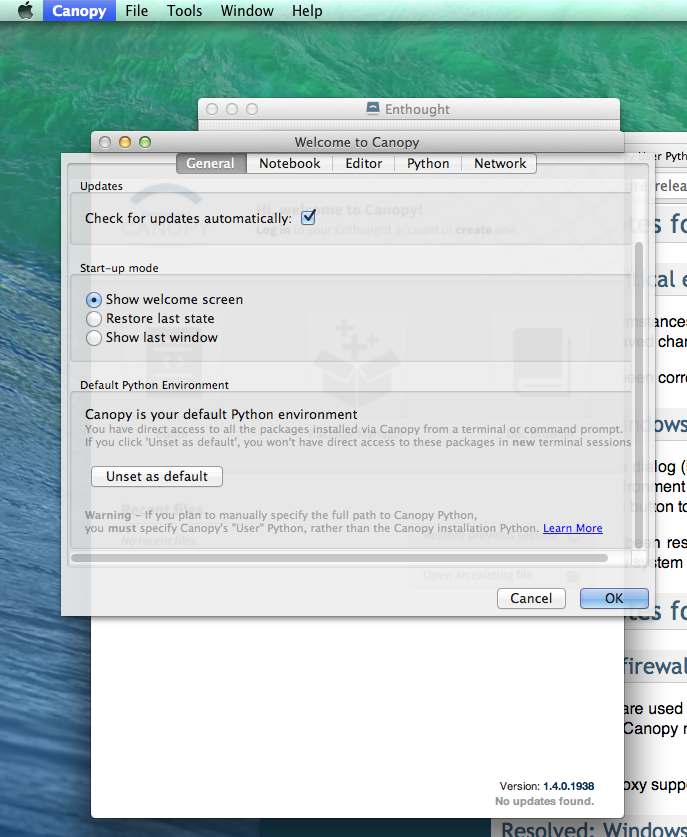
\includegraphics{enthought_as_default.png}


\subsection{Uninstalling Enthought Canopy}
\label{docfiles/install_dependencies:uninstalling-enthought-canopy}
The official Enthought gives suggestions on uninstalling \href{https://guide.macports.org/chunked/installing.macports.uninstalling.html}{here}.

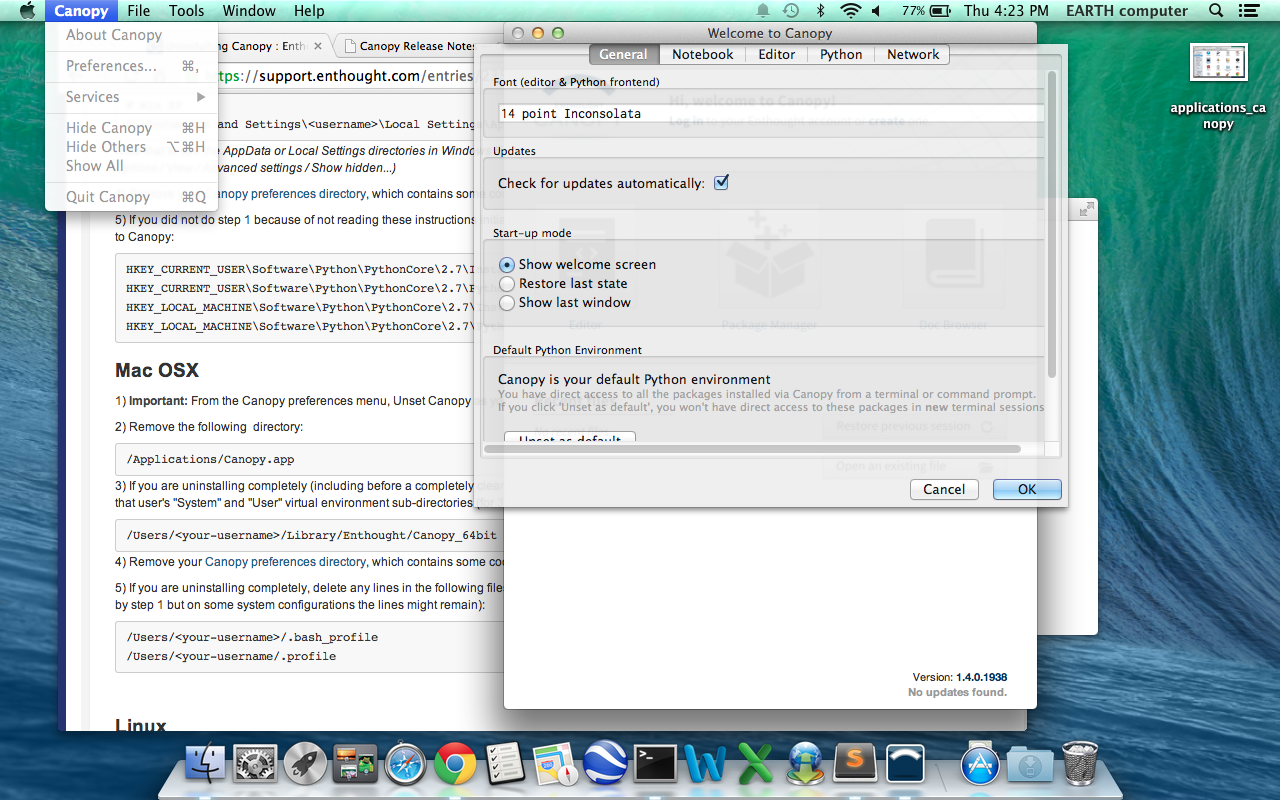
\includegraphics{canopy_preferences.png}

STEPS:
\begin{enumerate}
\item {} 
From the Canopy preferences menu, unset Canopy as your default Python.

\item {} 
For each Canopy user, delete the following directory which contains that user’s ``System'' and ``User'' virtual environment subdirections.

\item {} 
Delete Canopy from the Applications folder.

\item {} 
Clean up the hidden files. Delete anything referencing Canopy or Enthought in the hidden files, as evidence by referencing \code{ls -a} in your home directory. Check the \code{.bashrc} and \code{.profile} directories first. If Enthought is not completely gone, this happens if you call Python.

\item {} 
(Optional). Keep doing \code{which python} and cleaning the python files that show up, until \code{which python} gives you nothing when you type it in the terminal.

\end{enumerate}

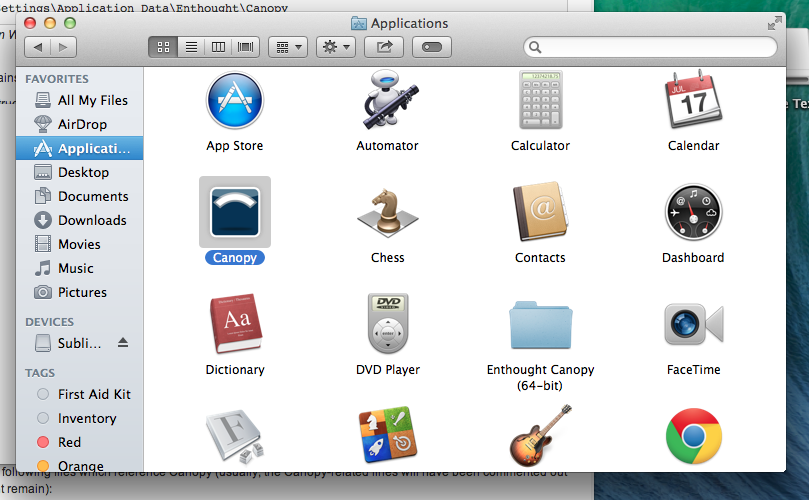
\includegraphics{applications_canopy.png}


\subsection{Path to python files not found}
\label{docfiles/install_dependencies:path-to-python-files-not-found}
After adding the path to your directory with scripts in \code{.bashrc}, you still need to source the \code{.bashrc} files in \code{.profile}, or the system may not find the directory. See here for more \href{http://publib.boulder.ibm.com/infocenter/pseries/v5r3/index.jsp?topic=/com.ibm.aix.baseadmn/doc/baseadmndita/prof\_file.htm}{details} to see how the profile file is sourced. Note that this one will override the file in \emph{/etc/profile}.

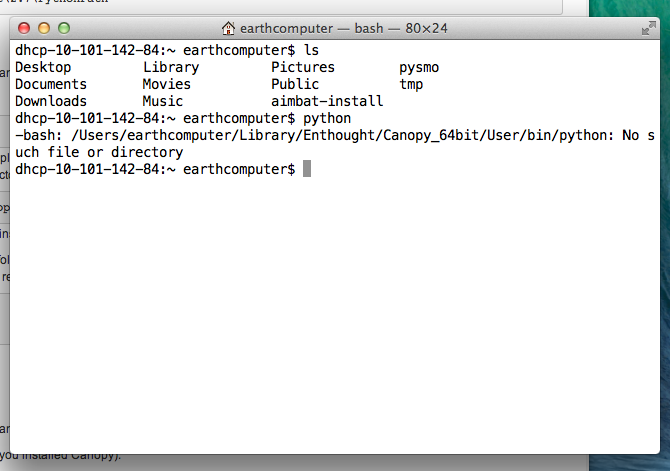
\includegraphics{residue.png}

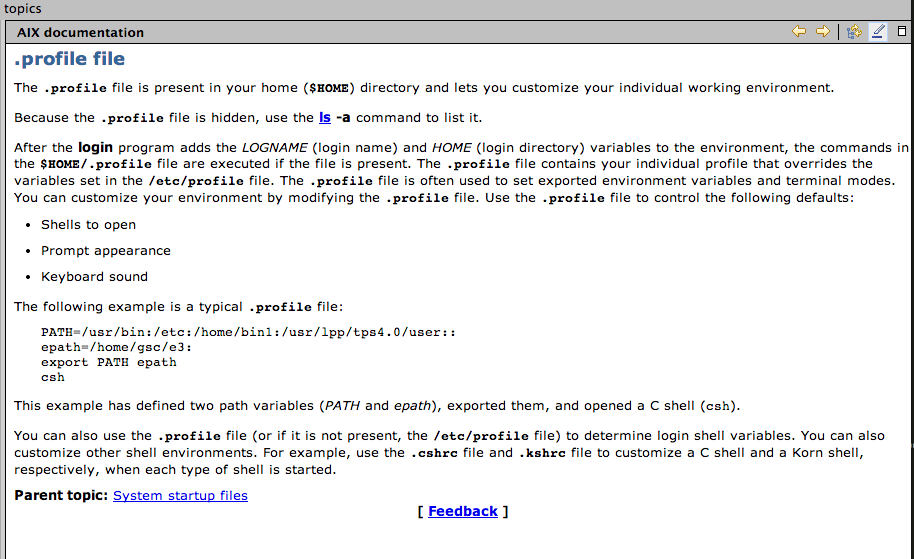
\includegraphics{profile_file.png}

\href{http://linux.die.net/man/1/bash}{This explanation} explains how the bashrc file is sourced.

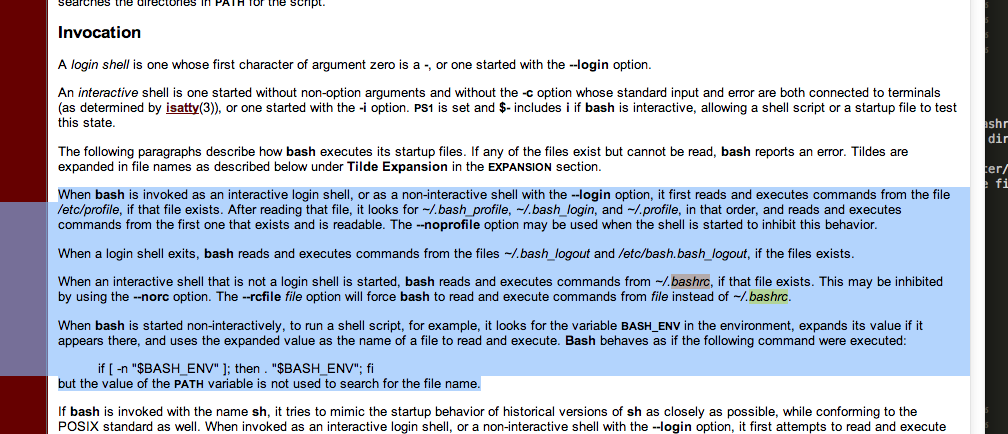
\includegraphics{bashrc_file.png}

This is what the bashrc and profile files should look like on your home directory:

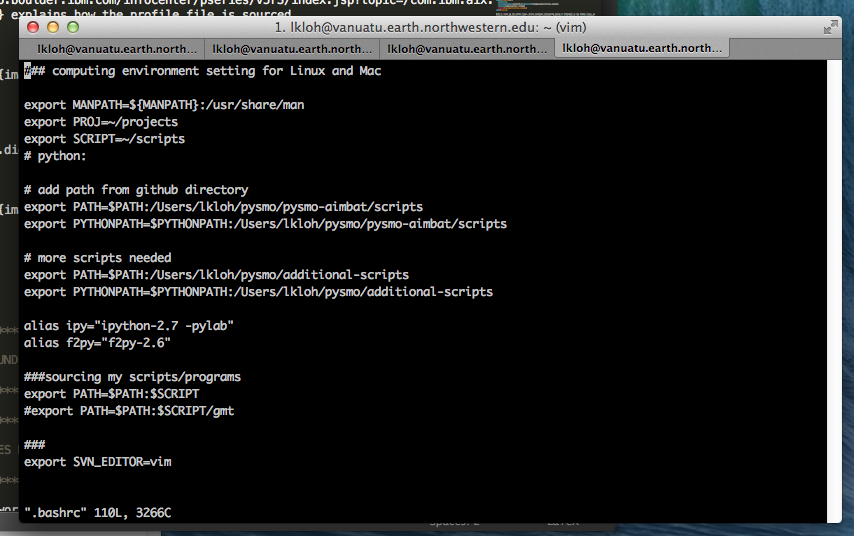
\includegraphics{bashrc_home.png}

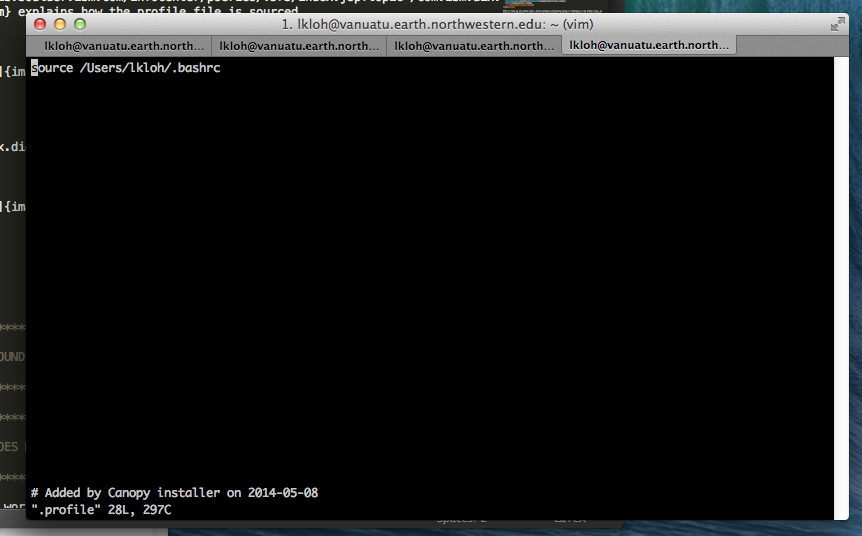
\includegraphics{profile_home.png}


\chapter{Installing AIMBAT}
\label{docfiles/install_aimbat::doc}\label{docfiles/install_aimbat:installing-aimbat}

\section{Getting the Packages}
\label{docfiles/install_aimbat:getting-the-packages}
AIMBAT is released as a sub-package of pysmo in the name of \code{pysmo.aimbat} along with another sub-package \code{pysmo.sac}. The latest stable release of AIMBAT is available for download at the \href{http://www.earth.northwestern.edu/~xlou/aimbat.html}{official project webpage}.

We are working on a new release of AIMBAT, available on \href{https://github.com/pysmo}{Github}. We are adding more features to make using AIMBAT more convenient, and fixing some bugs in the old code. Download \href{https://github.com/pysmo/aimbat}{pysmo.aimbat} and \href{https://github.com/pysmo/sac}{pysmo.sac} from Github. You will now have two folders called \code{aimbat} and \code{sac} respectively.

You may want to download \href{https://github.com/pysmo/data-example}{example code} to run AIMBAT on, as well.


\section{Where to install the packages}
\label{docfiles/install_aimbat:where-to-install-the-packages}
There are several options to install the packages. If you just want to use AIMBAT, it is best to store it somewhere where you would not touch the packages so easily, such as the Python \code{site-packages} directory. If you would like to make some changes to the Python code, it is best to store it somewhere pretty accessible, such as your \code{home} directory on your computer, or in \code{Documents}.


\subsection{Installing into the Python Site-Packages Directory}
\label{docfiles/install_aimbat:installing-into-the-python-site-packages-directory}
To find out where the Python Site-Packages Directory is, in the python console, do:

\begin{Verbatim}[commandchars=\\\{\}]
\PYG{k+kn}{import} \PYG{n+nn}{site}\PYG{p}{;}
\PYG{n}{site}\PYG{o}{.}\PYG{n}{getsitepackages}\PYG{p}{(}\PYG{p}{)}
\end{Verbatim}

Whatever is output is obtained, lets call it \code{\textless{}pkg-install-dir\textgreater{}}. Make a directory called \code{pysmo}, and place the sac and aimbat directories inside \code{\textless{}pkg-install-dir\textgreater{}/pysmo}.


\subsection{Installing into the home directory}
\label{docfiles/install_aimbat:installing-into-the-home-directory}
Open your terminal. Type \code{open .} and that will open your home directory. Transfer the \code{aimbat} and \code{sac} repositories inside there.


\section{Building the Pysmo Packages}
\label{docfiles/install_aimbat:building-the-pysmo-packages}
You need to be an administrator on the computer you are installing AIMBAT in, as you need to run the commands with \code{sudo}.


\subsection{Building pysmo.sac}
\label{docfiles/install_aimbat:building-pysmo-sac}
Python module \code{Distutils} is used to write a setup.py script to build, distribute, and install \code{pysmo.sac}. cd into the \code{sac} directory on the command line and run:

\begin{Verbatim}[commandchars=\\\{\}]
sudo python setup.py build
sudo python setup.py install
\end{Verbatim}

If you successfully installed the sac module, in the python console, this should happen after you type:

\begin{Verbatim}[commandchars=\\\{\}]
\PYG{k+kn}{from} \PYG{n+nn}{pysmo} \PYG{k+kn}{import} \PYG{n}{sac}
\end{Verbatim}


\subsection{Installing pysmo.aimbat}
\label{docfiles/install_aimbat:installing-pysmo-aimbat}
Three sub-directories are included in the \code{aimbat} directory:
\begin{itemize}
\item {} 
\code{example}: Example SAC files

\item {} 
\code{scripts}: Python scripts to run at the command line

\item {} 
\code{src}: Python modules to install

\end{itemize}

The core cross-correlation functions are written in both Python/Numpy (\code{xcorr.py}) and Fortran (\code{xcorr.f90}). Therefore, we need to use Numpy’s \code{Distutils} module for enhanced support of Fortran extension. The usage is similar to the standard Disutils.

Note that some sort of Fortran compiler must already be installed first. Specify them in place of gfortran in the following commands.

cd into the directory the \code{aimbat} package was placed in, and type:

\begin{Verbatim}[commandchars=\\\{\}]
sudo python setup.py build \PYGZhy{}\PYGZhy{}fcompiler=gfortran
sudo python setup.py install
\end{Verbatim}

to install the \code{src} directory.

Add \code{\textless{}path-to-folder\textgreater{}/aimbat/scripts} to environment variable \code{PATH} in a shells start-up file for command line execution of the scripts. Inside the \code{.bashrc} file, add the lines

Bash Shell Users:

\begin{Verbatim}[commandchars=\\\{\}]
export PATH=\PYGZdl{}PATH:\PYGZlt{}path\PYGZhy{}to\PYGZhy{}folder\PYGZgt{}/aimbat/scripts
\end{Verbatim}

C Shell Users:

\begin{Verbatim}[commandchars=\\\{\}]
setenv PATH=\PYGZdl{}PATH:\PYGZlt{}path\PYGZhy{}to\PYGZhy{}folder\PYGZgt{}/aimbat/scripts
\end{Verbatim}

If AIMBAT has beenn installed, type \code{from pysmo import aimbat} in a Python shell, and no errors should appear.

If you have added the scripts right, typing part of the name of the script in the terminal should be sufficient to allow the system autocomplete the name.


\section{Example Data}
\label{docfiles/install_aimbat:example-data}
Get the repository \href{https://github.com/pysmo/data-example}{data-example} from Github. There is some example code inside \emph{data-example/example\_pkl\_files} that will be needed for later demonstrations.


\chapter{Upgrading AIMBAT}
\label{docfiles/upgrading_aimbat:upgrading-aimbat}\label{docfiles/upgrading_aimbat::doc}

\section{Getting the latest version}
\label{docfiles/upgrading_aimbat:getting-the-latest-version}
The latest version of AIMBAT, currently version 0.1.3, is hosted on the \href{https://github.com/pysmo}{pysmo repository} on Github. We will periodically be making updates to it.

To upgrade AIMBAT, first delete the old AIMBAT files on your computer.

Next, download the newest version of \href{https://github.com/pysmo/aimbat}{AIMBAT} and \href{https://github.com/pysmo/sac}{SAC} from github. Now, cd into the newest AIMBAT folder and run:

\begin{Verbatim}[commandchars=\\\{\}]
sudo python setup.py build \PYGZhy{}\PYGZhy{}fcompiler=gfortran
sudo python setup.py install
\end{Verbatim}

Also, cd into the newest SAC folder and run:

\begin{Verbatim}[commandchars=\\\{\}]
sudo python setup.py build
sudo python setup.py install
\end{Verbatim}

Now, go to the \emph{.profile} file and add the \emph{scripts} folder in the new AIMBAT version to your path.

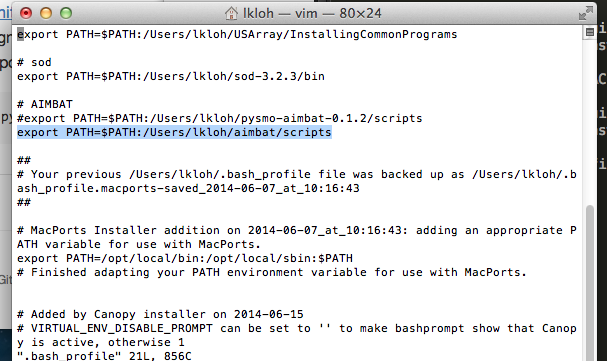
\includegraphics{upgrade-profile.png}


\section{Possible Issues}
\label{docfiles/upgrading_aimbat:possible-issues}
Some users have reported errors with upgrading. If there are any problems running the updated AIMBAT, try the following:

Get the location of the python \code{site-packages} directory by typing the following into the python console:

\begin{Verbatim}[commandchars=\\\{\}]
\PYG{k+kn}{import} \PYG{n+nn}{site}
\PYG{n}{site}\PYG{o}{.}\PYG{n}{getsitepackages}\PYG{p}{(}\PYG{p}{)}
\end{Verbatim}

The path to the site packages directory is highlighted in the figure below.

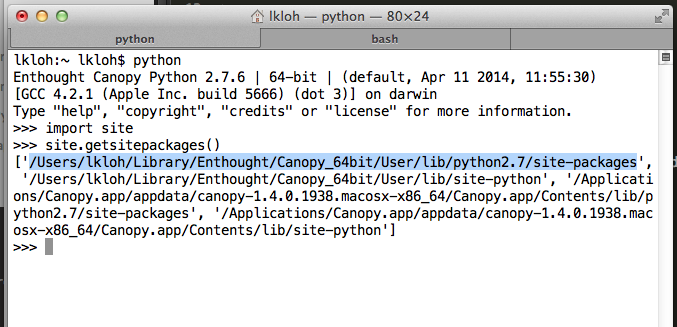
\includegraphics{get-site-package.png}

cd into the site-packages directory and remove all the folders with the word \code{pysmo} in their names by typing:

\begin{Verbatim}[commandchars=\\\{\}]
sudo rm \PYGZhy{}rf \PYGZlt{}psymo\PYGZhy{}folder\PYGZgt{}
\end{Verbatim}

Now, reinstall the new version of AIMBAT.


\chapter{Getting Data}
\label{docfiles/gettingData:getting-data}\label{docfiles/gettingData::doc}
Note: Not necessary if you already have your own set ways of obtaining data. This section is added for completeness.

There are several ways to obtain seismic data from \href{http://www.iris.edu/dms/nodes/dmc/data/types/waveform-data/}{IRIS} to input to AIMBAT. The authors used two ways to do it, and a further list of libraries for obtaining seismic data is provided in the sidebars \href{http://www.iris.edu/dms/nodes/dmc/data/types/waveform-data/}{here}.


\section{Obspy.fdsn for downloading data}
\label{docfiles/gettingData:obspy-fdsn-for-downloading-data}

\subsection{Installing Obspy}
\label{docfiles/gettingData:installing-obspy}
We recommend using Macports to install Obspy as detailed in the \emph{Installation} section \href{https://github.com/obspy/obspy/wiki}{here}. If you have installed Enthought Canopy:

\begin{Verbatim}[commandchars=\\\{\}]
sudo port install py27\PYGZhy{}obspy
\end{Verbatim}

should do it. If not, installing with \href{https://github.com/obspy/obspy/wiki/Installation-on-OS-X-using-Homebrew}{Homebrew} also seems to work.


\subsection{Did the installation work?}
\label{docfiles/gettingData:did-the-installation-work}
If installation has worked, \emph{close the terminal} you used to install Obspy on, and then open it again. Now, open the Python terminal in a new terminal, and type:

\begin{Verbatim}[commandchars=\\\{\}]
\PYG{k+kn}{import} \PYG{n+nn}{obspy}
\end{Verbatim}

If there are no errors, your installation has worked.


\subsection{Using Obspy}
\label{docfiles/gettingData:using-obspy}
Use the \href{http://docs.obspy.org/packages/obspy.fdsn.html\#}{Obspy FDSN} Web service client for Obspy in Python. Once you have done so, check out the \href{http://docs.obspy.org/packages/obspy.sac.html}{SAC-Input Output} libraries for loading the data to Python and saving it as SAC or Pickle files.


\section{Standing Order for Data}
\label{docfiles/gettingData:standing-order-for-data}
Note: NOT needed for AIMBAT, but important to know about as it is a commonly used package for downloading seismic data with the user's specifications. Although Obspy also offers was to download seismic data from IRIS, SOD allows for better fine-tuning of data obtained.

From the \href{http://www.seis.sc.edu/index.html}{SOD} website:
\begin{quote}

Standing Order for Data, is a framework to define rules to select seismic events, stations, and data. It then allows you to apply processing to the events, stations, and data and currently contains a large set of rules that allow you to select with great precision in these items. The processes mainly consist of simple data transformation and retrieval, but SOD defines hooks to allow you to cleanly insert your own processing steps, either written in Java or an external program.
\end{quote}


\subsection{Installing SOD}
\label{docfiles/gettingData:installing-sod}
First, download \href{http://www.seis.sc.edu/index.html}{SOD}.

Once you have gotten the folder for SOD, put it somewhere where you won't touch it too much. What I did was put the SOD folder in my home directory, though other places are acceptable as well, as long as its not too easy to delete it by accident.

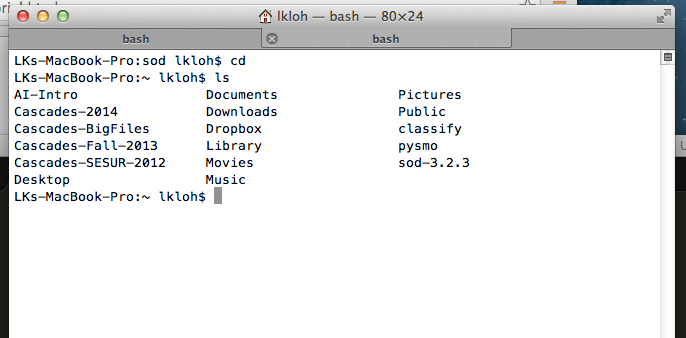
\includegraphics{sod_location.png}

Once you have it there, get the path to the sod folder's bin and put it in your path folder.

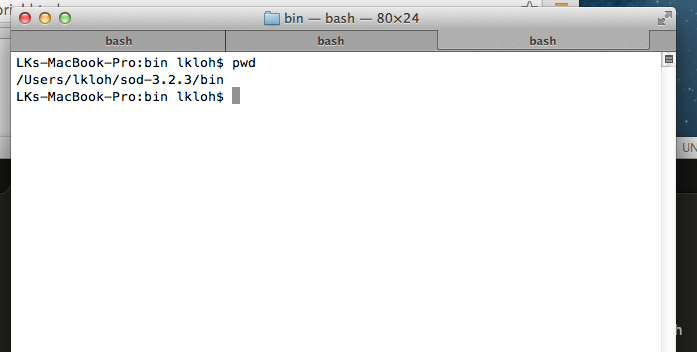
\includegraphics{path_to_sod_bin.png}

Inside my home directory's bash profile (you get the by typing \emph{cd}), you put the path to \emph{sod-3.2.3/bin} by adding in either the \emph{bash} or \emph{bash\_profile} or \emph{profile} files.


\subsection{Example SOD recipe}
\label{docfiles/gettingData:example-sod-recipe}
Inside the repository \href{https://github.com/pysmo/data-example}{data-example}, there is a folder \emph{sod\_requests}. The file within it called \emph{sod\_request.xml}, which is available \href{https://github.com/pysmo/data-example/blob/master/sod\_requests/sod\_request.xml}{here}, is an example of a sod request recipe that will download data from IRIS. To run it, cd into the folder containing \emph{sod\_request.xml}, and do:

\begin{Verbatim}[commandchars=\\\{\}]
sod sod\PYGZus{}request.xml
\end{Verbatim}

Downloading the data (output as SAC files) may take a while. This receipt filters the data, and outputs the folders \emph{processedSeismograms} and \emph{seismograms}, which container the filtered and unfiltered data.


\chapter{SAC Input/Output procedures for AIMBAT}
\label{docfiles/sacioAIMBAT:sac-input-output-procedures-for-aimbat}\label{docfiles/sacioAIMBAT::doc}
Once you have downloaded


\section{Converting from SAC to PKL files}
\label{docfiles/sacioAIMBAT:converting-from-sac-to-pkl-files}
Place the SAC files you want to convert to a pickle (PKL) file into the same folder. Suppose for instance, they are BHZ channels. Note that the SAC files must be of the same channel. cd into that folder, and run:

\begin{Verbatim}[commandchars=\\\{\}]
sac2pkl.py \PYGZhy{}s *.BHZ.sac
\end{Verbatim}

The output should be a PKL file in the same folder as the sac files.

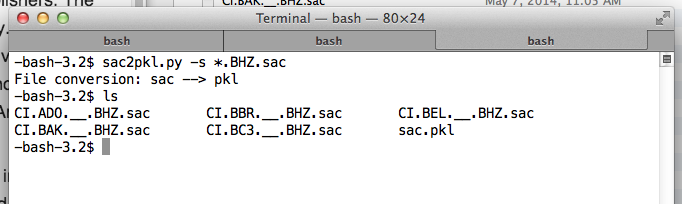
\includegraphics{sac_to_pkl_conversion.png}


\section{Converting from PKL to SAC files}
\label{docfiles/sacioAIMBAT:converting-from-pkl-to-sac-files}
Note: Not available for \emph{aimbat-stable}.

cd into the folder containing the PKL file that you wish to convert into SAC files, and run:

\begin{Verbatim}[commandchars=\\\{\}]
sac2pkl.py \PYGZhy{}\PYGZhy{}p2s \PYGZlt{}name\PYGZhy{}of\PYGZhy{}file\PYGZgt{}.pkl
\end{Verbatim}

The SAC files contained within will output into the same folder as the PKL file is stored in,

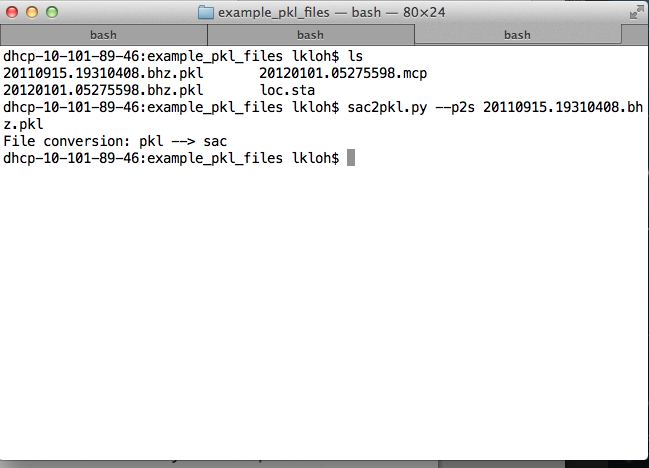
\includegraphics{pkl_to_sac_conversion.png}


\chapter{Filtering Data}
\label{docfiles/filteringData::doc}\label{docfiles/filteringData:filtering-data}
There are several options for filtering data. \href{http://www.iris.edu/files/sac-manual/}{SAC} offers several ways to filter data, which are not discussed here. You could also do so when downloading data using SOD. Alternatively, you could filter data in AIMBAT.


\section{Filtering GUI}
\label{docfiles/filteringData:filtering-gui}
To filter data, once you have imported the files to run into the GUI, hit the \code{filter} button to bring up the filtering GUI. The figure on top shows the results of the signal plotted against time before and after filtering with a \href{http://en.wikipedia.org/wiki/Butterworth\_filter}{butterworth filter}.

You can adjust the corner frequencies used on the figure on the lower corner. The defaults used here are:

\begin{tabulary}{\linewidth}{|L|L|}
\hline
\textsf{\relax 
Variable
} & \textsf{\relax 
Default
}\\
\hline
Order
 & 
2
\\

Filter Type
 & 
Bandpass
\\

Low Frequency
 & 
0.05 Hz
\\

High Frequency
 & 
0.25 Hz
\\
\hline\end{tabulary}


You can change the order and filter type by selecting the option you want. By clicking on the lower figure, you can select the low frequency and the high frequency you want. Click \code{apply} to filter the seismograms when you are satisfied with the filter paramters chosen.


\section{Saving Options}
\label{docfiles/filteringData:saving-options}
There are several options for saving the SAC header files of the seismograms you have chosen.

\begin{tabulary}{\linewidth}{|L|L|}
\hline
\textsf{\relax 
Button Title
} & \textsf{\relax 
What it does
}\\
\hline
Save Headers Only
 & 
Saves the SAC headers only
\\

Save Headers \& Filter Parameters
 & 
Saves the SAC headers and filter parameters used.
Those filter parameters will automatically the
next time the SAC headers are loaded in AIMBAT
\\

Save Headers \& Override Data
 & 
Save SAV headers and write in the filtered data
\\
\hline\end{tabulary}



\chapter{Analyzing Data}
\label{docfiles/analyzingData:analyzing-data}\label{docfiles/analyzingData::doc}

\section{Seismic Analysis Code (SAC)}
\label{docfiles/analyzingData:seismic-analysis-code-sac}
AIMBAT uses \href{http://www.iris.edu/files/sac-manual/}{Seismic Analysis Code (SAC)} formatting for some of the files it runs and outputs. To get SAC, you will need to fill out a software request form available on the IRIS website.


\chapter{Parameter Configuration}
\label{docfiles/parameterConfiguration:parameter-configuration}\label{docfiles/parameterConfiguration::doc}

\section{Backend}
\label{docfiles/parameterConfiguration:backend}
\href{http://matplotlib.org/contents.html}{Matplotlib} works with six GUI (Graphical User Interface) toolkits:
\begin{enumerate}
\item {} 
WX

\item {} 
Tk

\item {} 
Qt(4)

\item {} 
FTK

\item {} 
Fltk

\item {} 
macosx

\end{enumerate}

The GUI of AIMBAT uses the following to support interactive plotting:
\begin{enumerate}
\item {} 
\href{http://matplotlib.org/api/widgets\_api.html}{GUI neutral widgets}

\item {} 
\href{http://matplotlib.org/users/event\_handling.html}{GUI neutral event handling API (Application Programming Interface)}

\end{enumerate}

AIMBAT uses the default toolkit \code{Tk} and backend \code{TkAgg}.

Visit these pages for an \href{http://matplotlib.org/faq/usage\_faq.html\#what-is-a-backend}{explanation of the backend} and \emph{how to customize it \textless{}http://matplotlib.org/users/customizing.html\#customizing-matplotlib\textgreater{}}.


\section{Configuration File}
\label{docfiles/parameterConfiguration:configuration-file}
Other parameters for the package can be set up by a configuration file \code{ttdefaults.conf}, which is interpreted by the module ConfigParser. This configuration file is searched in the following order:
\begin{enumerate}
\item {} 
file \code{ttdefaults.conf} in the current working directory

\item {} 
file \code{.aimbat/ttdefaults.conf} in your \code{HOME} directory

\item {} 
a file specified by environment variable \code{TTCONFIG}

\item {} 
file \code{ttdefaults.conf} in the directory where AIMBAT is installed

\end{enumerate}

Python scripts in the \code{\textless{}pkg-install-dir\textgreater{}/pysmo-aimbat-0.1.2/scripts} can be executed from the command line. The command line arguments are parsed by the optparse module to improve the scripts' exibility. If conflicts existed, the command line options override the default parameters given in the configuration file \code{ttdefaults.conf}. Run the scripts with the \code{-h} option for the usage messages.


\subsection{Example of AIMBAT configuration file \emph{ttdefaults.conf}}
\label{docfiles/parameterConfiguration:example-of-aimbat-configuration-file-ttdefaults-conf}
\begin{tabulary}{\linewidth}{|L|L|}
\hline
\textsf{\relax 
ttdefaults.conf
} & \textsf{\relax 
Description
}\\
\hline
{[}sacplot{]}
 & \\

colorwave = blue
 & 
Color of waveform
\\

colorwavedel = gray
 & 
Color of waveform which is deselected
\\

colortwfill = green
 & 
Color of time window fill
\\

colortwsele = red
 & 
Color of time window selection
\\

alphatwfill = 0.2
 & 
Transparency of time window fill
\\

alphatwsele = 0.6
 & 
Transparency of time window selection
\\

npick = 6
 & 
Number of time picks (plot picks: t0-t5)
\\

pickcolors = kmrcgyb
 & 
Colors of time picks
\\

pickstyles
 & 
Line styles of time picks (use second one if ran out of color)
\\

figsize = 8 10
 & 
Figure size for \emph{plotphase.py}
\\

rectseis = 0.1 0.06 0.76 0.9
 & 
Axes rectangle size within the figure
\\

minspan = 5
 & 
Minimum sample points for SpanSelector to select time window
\\

srate = -1
 & 
Sample rate for loading SAC data.
Read from first file if srate \textless{} 0
\\
\hline\end{tabulary}


\begin{tabulary}{\linewidth}{|L|L|}
\hline
 \multicolumn{2}{|l|}{\textsf{\relax 
{[}sachdrs{]}
}}\\
\hline
twhdrs = user8 user9
 & 
SAC headers for time window beginning and ending
\\

ichdrs = t0 t1 t2
 & 
SAC headers for ICCS time picks
\\

mchdrs = t2 t3
 & 
SAC headers for MCCC input and output time picks
\\

hdrsel = kuser0
 & 
SAC header for seismogram selection status
\\

qfactors = ccc snr coh
 & 
Quality factors: cross-correlation coefficient,
signal-to-noise ratio, time domain coherence
\\

qheaders = user0 user1 user2
 & 
SAC Headers for quality factors
\\

qweights = 0.3333 0.3333 0.3333
 & 
Weights for quality factors
\\
\hline\end{tabulary}


\begin{tabular}{|p{0.475\linewidth}|p{0.475\linewidth}|}
\hline
\textsf{\relax 
{[}iccs{]} or Align/Refine
} & \textsf{\relax }\\
\hline
srate = -1
 & 
Sample rate for loading SAC data. Read from first file if srate \textless{} 0
\\

xcorr\_modu = xcorrf90
 & 
Module for calculating cross-correlation:
xcorr for Numpy or xcorrf90 for Fortran
\\

xcorr\_func = xcorr\_fast
 & 
Function for calculating cross-correlation
\\

shift = 10
 & 
Sample shift for running coarse cross-correlation
\\

maxiter = 10
 & 
Maximum number of iteration
\\

convepsi = 0.001
 & 
Convergence criterion: epsilon
\\

convtype = coef
 & \begin{description}
\item[{Type of convergence criterion: coef for correlation coefficient,}] \leavevmode
or resi for residual

\end{description}
\\

stackwgt = coef
 & 
Weight each trace when calculating array stack
\\

fstack = fstack.sac
 & 
SAC file name for the array stack
\\
\hline\end{tabular}


\begin{tabulary}{\linewidth}{|L|L|}
\hline
\textsf{\relax 
{[}mccc{]}
} & \textsf{\relax }\\
\hline
srate = -1
 & 
Sample rate for loading SAC data.
Read from first file if srate \(< 0\)
\\

ofilename = mc
 & 
Output file name of MCCC.
\\

xcorr\_modu = xcorrf90
 & 
Module for calculating cross-correlation:
xcorr for Numpy or xcorrf90 for Fortran
\\

xcorr\_func = xcorr\_faster
 & 
Function for calculating cross-correlation
\\

shift = 10
 & 
Sample shift for running coarse cross-correlation
\\

extraweight = 1000
 & 
Weight for the zero-mean equation in MCCC weighted lsqr solution
\\

lsqr = nowe
 & 
Type of lsqr solution: no weight
\\

\#lsqr = lnco
 & 
Type of lsqr solution: weighted by correlation coefficient,
solved by lapack
\\

\#lsqr = lnre
 & 
Type of lsqr solution: weighted by residual, solved by lapack
\\

rcfile = .mcccrc
 & 
Configuration file for MCCC parameters (deprecated)
\\

evlist = event.list
 & 
File for event hypocenter and origin time (deprecated)
\\
\hline\end{tabulary}


\begin{tabulary}{\linewidth}{|L|L|}
\hline
\textsf{\relax 
signal
} & \textsf{\relax }\\
\hline
tapertype = hanning
 & 
Taper type
\\

taperwidth = 0.1
 & 
Taper width
\\
\hline\end{tabulary}



\chapter{SAC Data Access}
\label{docfiles/SACdataAccess:sac-data-access}\label{docfiles/SACdataAccess::doc}

\section{Python Object for SAC File}
\label{docfiles/SACdataAccess:python-object-for-sac-file}
The \code{pysmo.sac} package is developed to read and write individual SAC files.
The Python class \code{sacfile} of module \code{sacio} opens a SAC file and returns an object including data and all SAC header variables as its attributes. Modifications of object attributes are saved to file. It is written purely in Python so that it also runs with \href{http://www.jython.org}{Jython}.


\subsection{\emph{egsac.py}}
\label{docfiles/SACdataAccess:egsac-py}
The \code{\textless{}pkg-install-dir\textgreater{}/aimbat/scripts/egsac.py} script gives a simple example to read, resample and plot a seismogram using pysmo, Scipy and Matplotlib. You can type the codes in a Python/iPython shell, or run as a script in the data example directory \code{\textless{}pkg-install-dir\textgreater{}/data-example/example\_pkl\_files/Event\_2011.09.15.19.31.04.080}, hereafter refered to as \emph{\textless{}example-event-dir\textgreater{}}.

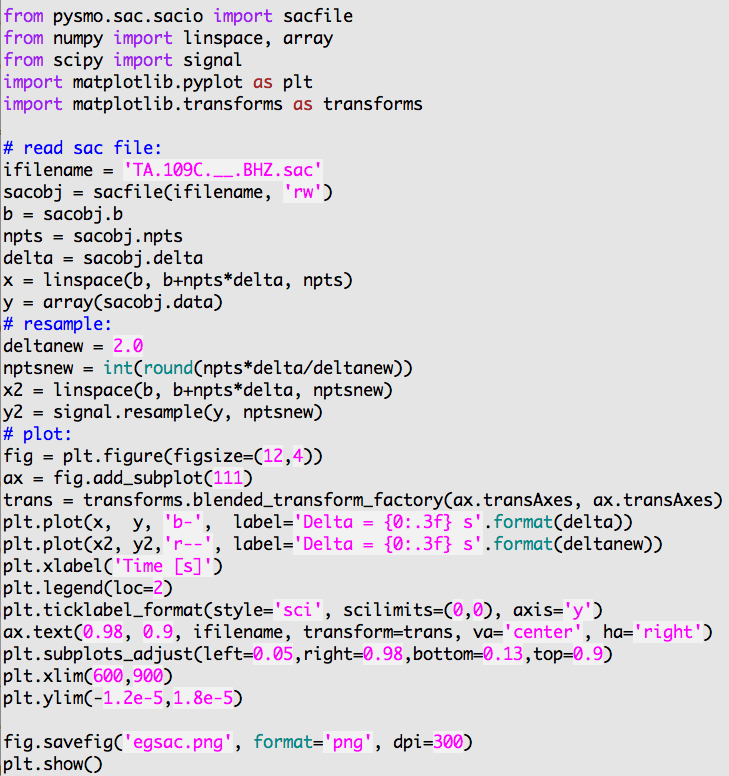
\includegraphics{prog-egsac.png}


\subsection{Resampling Seismograms}
\label{docfiles/SACdataAccess:resampling-seismograms}
In this example, a SAC file named \code{TA.109C.\textbackslash{}\_\textbackslash{}\_.BHZ.sac} is read in as a sacfile object. The time array is calculated from SAC headers.  The data array is resampled from interval 0.025 to 2.0 seconds using Scipy's signalprocessing module.

Add the following codes to write the resampled seismogram to file \code{TA.109C.\textbackslash{}\_\textbackslash{}\_.BHZ.sac}:

\begin{Verbatim}[commandchars=\\\{\}]
\PYG{n}{sacobj}\PYG{o}{.}\PYG{n}{delta} \PYG{o}{=} \PYG{n}{deltanew}
\PYG{n}{sacobj}\PYG{o}{.}\PYG{n}{npts} \PYG{o}{=} \PYG{n}{nptsnew}
\PYG{n}{sacobj}\PYG{o}{.}\PYG{n}{data} \PYG{o}{=} \PYG{n}{y2}
\end{Verbatim}

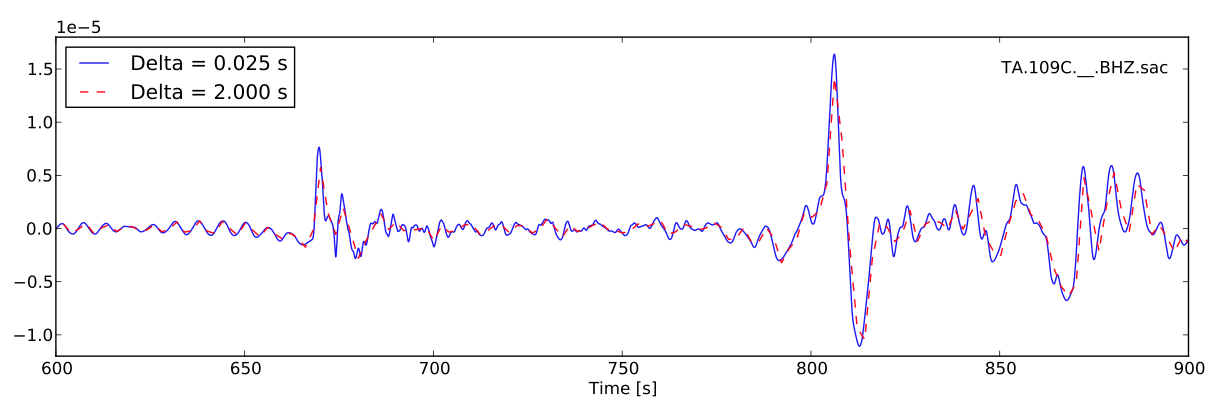
\includegraphics{egsac-109c.png}


\section{Python Pickle for SAC Files}
\label{docfiles/SACdataAccess:python-pickle-for-sac-files}
The \code{pysmo.sacio} module converts SAC files to \code{sacfile} objects. Any modification of the objects are instantly written to files. In data processing, the user may want to abandon changes made earlier, which brings the need of a buffer for the \code{sacfile} objects.

The \code{SacDataHdrs} class in the \code{pysmo.aimbat.sacpickle} module is written on top of \code{pysmo.sacio} to serves this purpose by reading a SAC file and returning a \code{sacdh} object that is very similar of the \code{sacfile} object. Essentially, the \code{sacdh} object is a copy of the the \code{sacfile} object in the memory, except that SAC headers `t0-t9', `user0-user9', `kuser0-kuser2' are saved in three Python lists.

A \code{gsac} object of the \code{SacGroup} class consists of a group of \code{sacdh} objects from event-based SAC data files, earthquake hypocenter information and station locations.
An additional step is required to save changes in the \code{gsac} object to files.

In order to avoid frequent SAC file I/O, the \code{pickle/cPickle} module is used for serializing and de-serializing the \code{gsac} object structure. Thus the data processing efficiency is improved because reading and writing of SAC files are done only once each before and after data processing. Script \code{sac2pkl.py} does the conversions between SAC files and Python pickles.

Its usage message can be printed out by running at command line:

\begin{Verbatim}[commandchars=\\\{\}]
\PYG{n}{sac2pkl}\PYG{o}{.}\PYG{n}{py} \PYG{o}{\PYGZhy{}}\PYG{n}{h}
\end{Verbatim}

and the result is displayed in the figure below. For example, in the data example directory \code{\textless{}example-event-dir\textgreater{}}, run:

\begin{Verbatim}[commandchars=\\\{\}]
sac2pkl.py \PYGZhy{}s *Z \PYGZhy{}o 20110915.19310408.bhz.pkl \PYGZhy{}d 0.025
\end{Verbatim}

to read 163 vertical component seismograms at a sample interval of 0.025 s and convert to a \code{gsac} object which is saved in the pickle file \code{20110915.19310408.bhz.pkl}.

To save disk space, compressed pickle files in \code{gz} and \code{bz2} formats can be generated by:

\begin{Verbatim}[commandchars=\\\{\}]
sac2pkl.py \PYGZhy{}s *Z \PYGZhy{}o 20110915.19310408.bhz.pkl \PYGZhy{}d 0.025 \PYGZhy{}z gz
sac2pkl.py \PYGZhy{}s *Z \PYGZhy{}o 20110915.19310408.bhz.pkl \PYGZhy{}d 0.025 \PYGZhy{}z bz2
\end{Verbatim}

at the cost of more CPU time.

After processing, run:

\begin{Verbatim}[commandchars=\\\{\}]
sac2pkl.py 20110915.19310408.bhz.pkl \PYGZhy{}p
\end{Verbatim}

to convert the pickle file to SAC files.

..image:: SACdataAccess/help-sac2pkl

See the doc string of \code{pysmo.aimbat.sacpickle} by typing in a python console:

\begin{Verbatim}[commandchars=\\\{\}]
from pysmo.aimbat import sacpickle
print sacpickle.\PYGZbs{}\PYGZus{}\PYGZbs{}\PYGZus{}doc\PYGZbs{}\PYGZus{}\PYGZbs{}\PYGZus{}
\end{Verbatim}

and also the documentation on \href{http://docs.python.org/library/pickle.html}{pickle} for more information about the Python data structure, pickling and unpickling.


\section{SAC Plotting and Phase Picking}
\label{docfiles/SACdataAccess:sac-plotting-and-phase-picking}
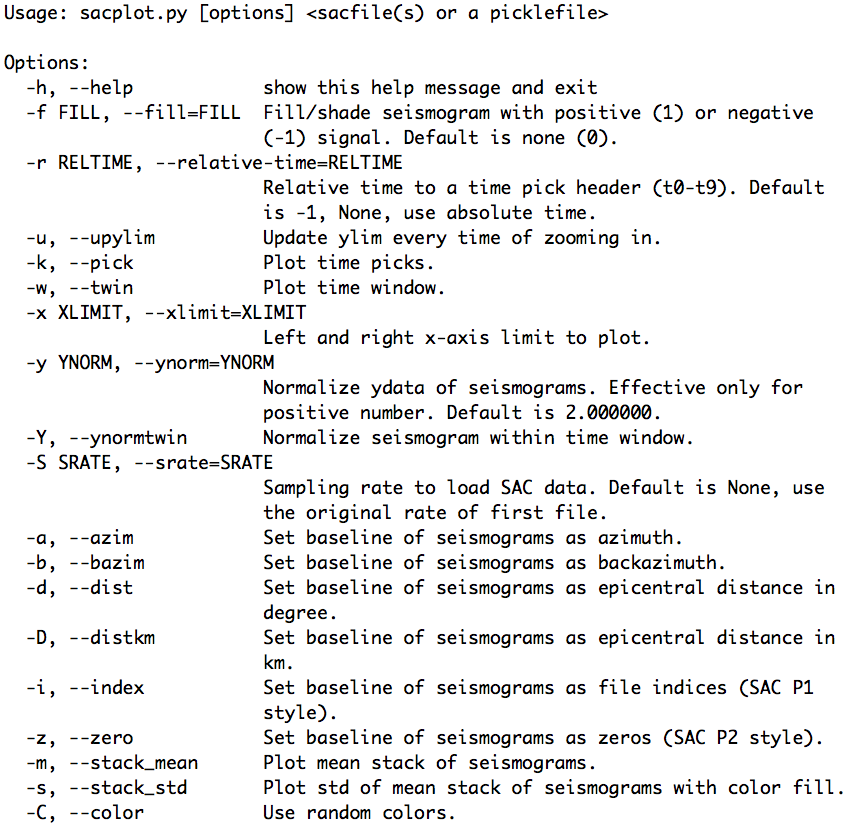
\includegraphics{help-sacplot.png}

SAC plotting and phase picking functionalities are replicated and enhanced based on the GUI neutral widgets (such as Button and SpanSelector) and the event (keyboard and mouse events such as \code{key\textbackslash{}\_press\textbackslash{}\_event} and \code{mouse\textbackslash{}\_motion\textbackslash{}\_event} handling API of Matplotlib.

They are implemented in two modules \code{pysmo.aimbat.plotphase} and \code{pysmo.aimbat.pickphase}, which are used by corresponding scripts \code{sacplot.py} and \code{sacppk.py} executable at command line. Their help messages are displayed in the figures below.

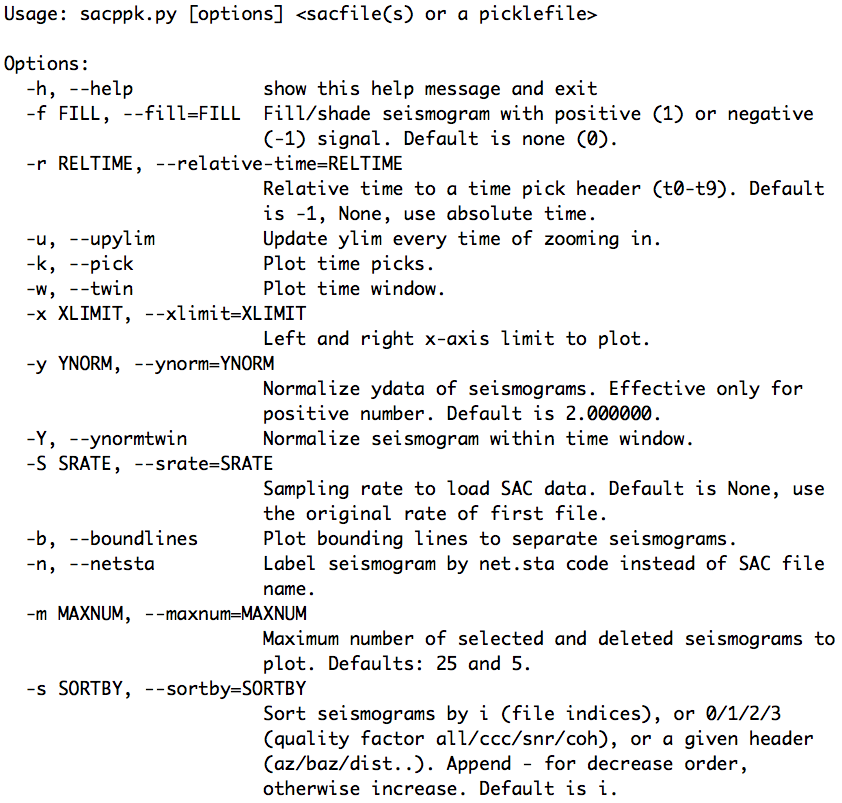
\includegraphics{help-sacppk.png}

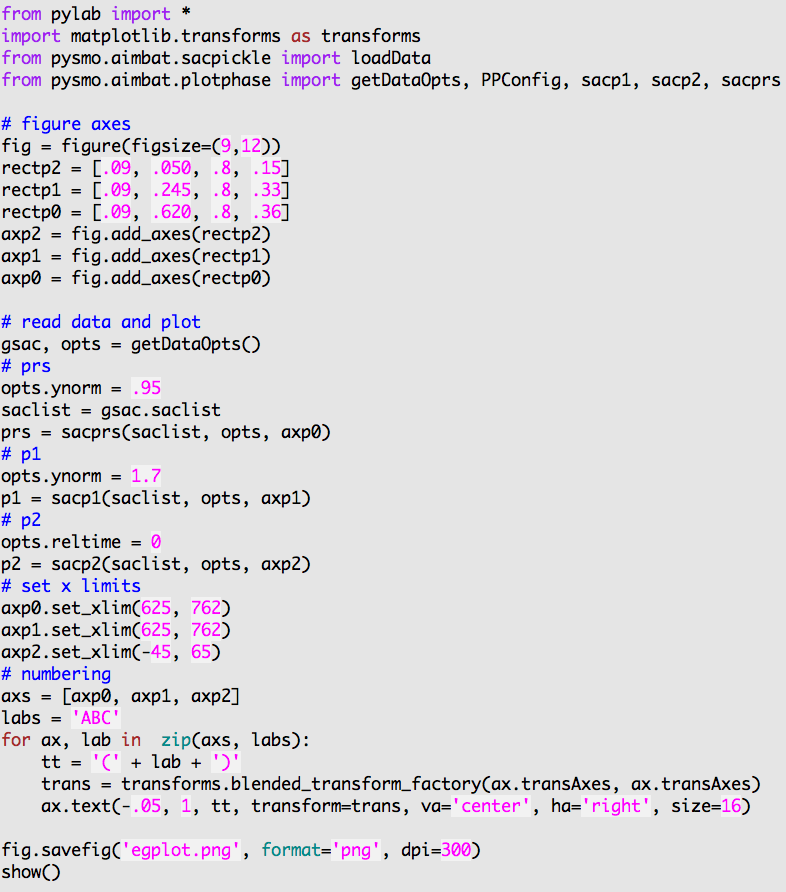
\includegraphics{prog-egplot.png}


\subsection{SAC Plotting}
\label{docfiles/SACdataAccess:sac-plotting}
Options ``-i, -z, -d, -a, and -b'' of \code{sacplot.py} set the seismogram plotting baseline as file index, zero, epicentral distance in degrees, azimuth, and back-azimuth, respectively.
The user can run \code{sacplot.py} directly with the options, or run individual scripts
\code{sacp1.py}, \code{sacp2.py}, \code{sacprs.py}, \code{sacpaz.py}, and \code{sacpbaz.py} which preset the baseline options and plot seismograms in SAC p1 style, p2 style, record section, and relative to azimuth and back-azimuth. The following commands are equivalent:

\begin{Verbatim}[commandchars=\\\{\}]
\PYG{n}{sacplot}\PYG{o}{.}\PYG{n}{py} \PYG{o}{\PYGZhy{}}\PYG{n}{i}\PYG{p}{,} \PYG{n}{sacp1}\PYG{o}{.}\PYG{n}{py}
\PYG{n}{sacplot}\PYG{o}{.}\PYG{n}{py} \PYG{o}{\PYGZhy{}}\PYG{n}{z}\PYG{p}{,} \PYG{n}{sacp2}\PYG{o}{.}\PYG{n}{py}
\PYG{n}{sacplot}\PYG{o}{.}\PYG{n}{py} \PYG{o}{\PYGZhy{}}\PYG{n}{d}\PYG{p}{,} \PYG{n}{sacprs}\PYG{o}{.}\PYG{n}{py}
\PYG{n}{sacplot}\PYG{o}{.}\PYG{n}{py} \PYG{o}{\PYGZhy{}}\PYG{n}{a}\PYG{p}{,} \PYG{n}{sacpaz}\PYG{o}{.}\PYG{n}{py}
\PYG{n}{sacplot}\PYG{o}{.}\PYG{n}{py} \PYG{o}{\PYGZhy{}}\PYG{n}{b}\PYG{p}{,} \PYG{n}{sacpbaz}\PYG{o}{.}\PYG{n}{py}
\end{Verbatim}

Input data files need to be supplied to the scripts in the form of either a list of SAC files or a pickle file which includes multiple SAC files. For example, a \code{bhz.pkl} file is generated from 22 vertical component seismograms \code{TA.{[}1-K{]}*Z} by running:

\begin{Verbatim}[commandchars=\\\{\}]
sac2pkl.py TA.[1\PYGZhy{}K]*BHZ \PYGZhy{}o bhz.pkl \PYGZhy{}d0.025
\end{Verbatim}

in the data example directory \code{\textless{}example-event-dir\textgreater{}}. Then the two commands are equivalent:

\begin{Verbatim}[commandchars=\\\{\}]
sacp1.py TA.[1\PYGZhy{}K]*Z
\end{Verbatim}

or:

\begin{Verbatim}[commandchars=\\\{\}]
sacp1.py bhz.pkl
\end{Verbatim}

For large number of seismograms, the pickle file is suggested because of faster loading.

Besides using the standard \code{sacplot.py} script, the user can modify its \code{getAxes} function in your own script to customize figure size and axes attributes. Script \code{egplot.py} is such an example in which SAC p1, p2 styles and record section plotting are drawn in three axes in the same figure canvas. Run:

\begin{Verbatim}[commandchars=\\\{\}]
egplot.py TA.[1\PYGZhy{}K]*Z  \PYGZhy{}f1 \PYGZhy{}C
\end{Verbatim}

at command line to produce the figure below.

..image:: SACdataAccess/egplot.png

The ``-C'' option uses random color for each seismogram.
The ``-f1'' option fills the positive signals of waveform with less transparency.
In the script, ``opts.ynorm'' sets the waveform normalization and ``opts.reltime=0'' sets the time axis relative to time pick t0.

An improvement over SAC is that the program outputs the filename when the seismogram is clicked on by the mouse. This is enabled by the event handling API and is mostly introduced for use in SAC p2 style plotting when seismograms are plotted on top of each other. It is especially useful when a large number of seismograms create difficulties in labeling.

Another improvement is easier window zooming enabled by the SpanSelector widget and the event handling API. Select a time span by mouse clicking and dragging to zoom in a waveform section.
Press the `z' key to zoom out to the previous time range.


\section{SAC Phase Picking}
\label{docfiles/SACdataAccess:sac-phase-picking}
SAC plotting (\code{pysmo.aimbat.plotphase}) does not involve change in data files but phase picking (\code{pysmo.aimbat.pickphase}) does. A GUI is built for user to interactively pick phase arrival times. The figure below is an example screen shot running:

\begin{Verbatim}[commandchars=\\\{\}]
sacppk.py 20110915.19310408.bhz.pkl \PYGZhy{}w
\end{Verbatim}

in the data example directory \code{\textless{}example-event-dir\textgreater{}}.

Following SAC convention, the user can set a time pick by pressing the `t' key and number keys `0-9'. The x location of the mouse position is saved to corresponding SAC headers `t0-t9'.
Time window zooming in \code{pysmo.aimbat.pickphase} is implemented in the same way as in \code{pysmo.aimbat.plotphase} to replace SAC's combination of the `x' key and mouse click.
Zooming out key is set to `z' because the `o' key is used for another purpose by Matplotlib.
The filename printing out by mouse clicking feature is also available in \code{pysmo.aimbat.pickphase}.

A major improvement over SAC is picking a time window in addition to time picks.
Pressing the `w' key to save the current time axis range to two user-defined SAC header variables. A transparent green span is plotted within the time window, show in the figure below.

..image:: SACdataAccess/sacppk.png

Another major improvement involves quality control with convenient operations to (de)select seismograms. In the GUI in above, there are two divisions of selected and deleted seismograms.
Selected seismograms with a positive trace number are displayed with blue wiggles, while deleted seismograms with negative trace numbers are plotted in gray. The user can simply click on a certain seismogram to switch the selection status, either to exclude it or bring it back for inclusion. The trace selection status is stored in a user-defined SAC header variable.

In SAC, command \code{ppk p 10} plots 10 seismograms on each page. Pressing the `b' and `n' keys to navigate through pages. The number of seismograms plotted on each page is controlled by command line option:

\begin{Verbatim}[commandchars=\\\{\}]
\PYGZhy{}m maxsel maxdel
\end{Verbatim}

for \code{sacppk.py}. The \code{Prev} and \code{Next} Buttons are for page navigation and the \code{Save} Button saves the change in time picks and time window to files. The default values for maxsel and maxdel are 25 and 5, which means a maximum of 30 seismograms on each page.

In the figure displayed, there are 26 seismograms on the first page because only 1 seismogram is deleted. On the next page, there are 30 selected seismograms. To plot 50 seismograms on each page, run:

\begin{Verbatim}[commandchars=\\\{\}]
sacppk.py 20110915.19310408.bhz.pkl \PYGZhy{}w \PYGZhy{}m 45 5
\end{Verbatim}

and there would be 4 total pages and 13 seismograms on the last page.

To plot seismograms relative to time pick t0 and fill the positive and negative wiggles of waveform, run:

\begin{Verbatim}[commandchars=\\\{\}]
sacppk.py 20110915.19310408.bhz.pkl \PYGZhy{}w \PYGZhy{}r0 \PYGZhy{}f1
\end{Verbatim}

To sort seismograms by epicentral distance in increase and decrease orders, run:

\begin{Verbatim}[commandchars=\\\{\}]
sacppk.py 20110915.19310408.bhz.pkl \PYGZhy{}w \PYGZhy{}sdist
sacppk.py 20110915.19310408.bhz.pkl \PYGZhy{}w \PYGZhy{}sdist\PYGZhy{}
\end{Verbatim}

Sorting by azimuth and back-azimuth is similar:

\begin{Verbatim}[commandchars=\\\{\}]
sacppk.py 20110915.19310408.bhz.pkl \PYGZhy{}w \PYGZhy{}saz
sacppk.py 20110915.19310408.bhz.pkl \PYGZhy{}w \PYGZhy{}sbaz
\end{Verbatim}

The help message of the \code{iccs.py} script is shown below:

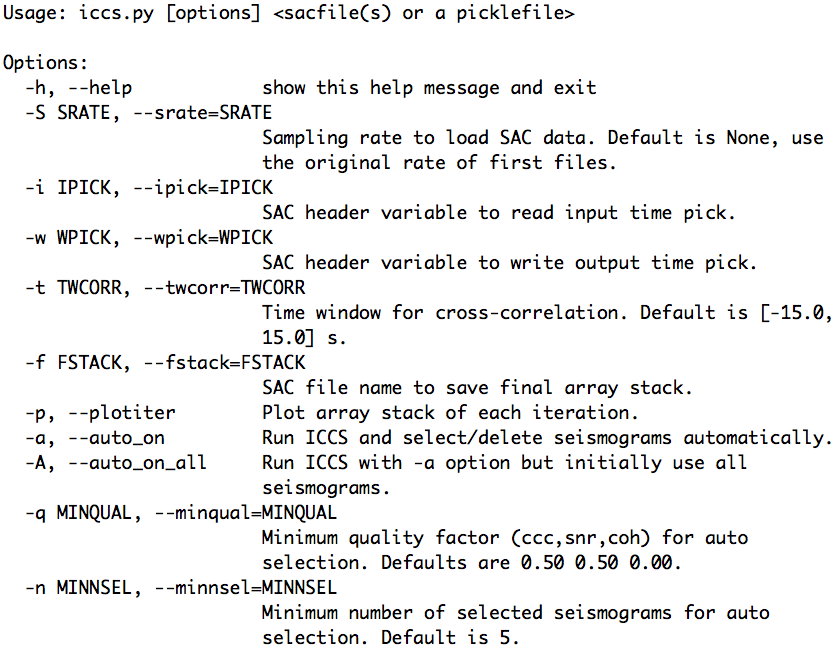
\includegraphics{help-iccs.png}

The help message of the \code{mccs.py} script is shown below:

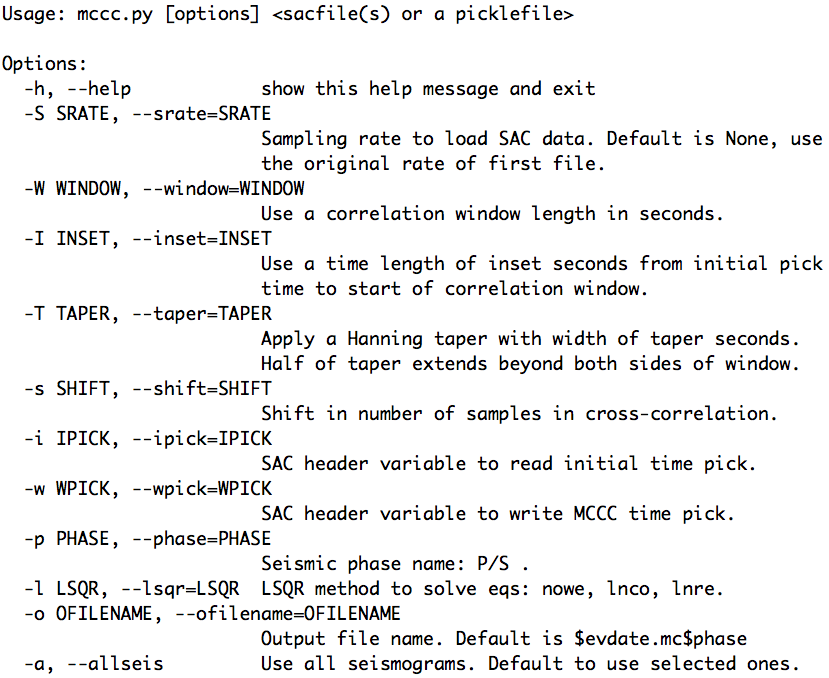
\includegraphics{help-mccc.png}


\chapter{Measuring Teleseismic Body Wave Arrival Times}
\label{docfiles/PickingTravelTimes::doc}\label{docfiles/PickingTravelTimes:measuring-teleseismic-body-wave-arrival-times}
The core idea in using AIMBAT to measure teleseismic body wave arrival times has two parts:
\begin{itemize}
\item {} 
automated phase alignment, to reduce user processing time, and

\item {} 
interactive quality control, to retain valuable user inputs.

\end{itemize}


\section{Automated Phase Alignment}
\label{docfiles/PickingTravelTimes:automated-phase-alignment}
The ICCS algorithm calculates an array stack from predicted time picks, cross-correlates each seismogram with the array stack to Find the time lags at maximum cross-correlation, then use the new time picks to update the array stack in an iterative process. The MCCC algorithm cross-correlates each possible pair of seismograms and uses a least-squares method to calculate an optimized set of relative arrival times. Our method is to combine ICCS and MCCC in a four-step procedure using four anchoring time picks \(_0T_i,\,_1T_i,\,_2T_i,\) and \(_3T_i\).
\begin{enumerate}
\item {} 
Coarse alignment by ICCS

\item {} 
Pick phase arrival at the array stack

\item {} 
Refined alignment by ICCS

\item {} 
Final alignment by MCCC

\end{enumerate}

The one-time manual phase picking at the array stack in step (b) allows the measurement of absolute arrival times. The detailed methodology and procedure can be found in {\hyperref[docfiles/citations:louvanderlee2013]{{[}LouVanDerLee2013{]}}}.


\begin{threeparttable}
\capstart\caption{Time picks and their SAC headers used in the procedure for measuring teleseismic body wave arrival times.}

\begin{tabular}{|p{0.136\linewidth}|p{0.136\linewidth}|p{0.136\linewidth}|p{0.136\linewidth}|p{0.136\linewidth}|p{0.136\linewidth}|p{0.136\linewidth}|}
\hline
 \multirow{2}{*}{
Step
} &  \multirow{2}{*}{
Algorithm
} &  \multicolumn{3}{l|}{
Input
} &  \multicolumn{2}{l|}{
Output
}\\
 & 
Time Window
 &  & 
Time Pick
 & 
Time Header
 & 
Time Pick
 & 
Time Header
\\
\begin{enumerate}
\item {} 
\end{enumerate}
 & 
ICCS
 & 
\(W_a\)
 & 
\(_0T_i\)
 & 
\textbf{T0}
 & 
\(_1T_i\)
 & 
\textbf{T1}
\\
\begin{enumerate}
\setcounter{enumi}{1}
\item {} 
\end{enumerate}
 & 
ICCS
 & 
\(W_b\)
 & 
\(_2T'_i\)
 & 
\textbf{T2}
 & 
\(_2T_i\)
 & 
\textbf{T2}
\\
\begin{enumerate}
\setcounter{enumi}{3}
\item {} 
\end{enumerate}
 & 
MCCS
 & 
\(W_b\)
 & 
\(_2T_i\)
 & 
\textbf{T2}
 & 
\(_3T_i\)
 & 
\textbf{T3}
\\
\hline\end{tabular}

\end{threeparttable}


The ICCS and MCCC algorithms are implemented in two modules \code{pysmo.aimbat.algiccs} and \code{pysmo.aimbat.algmccc}, and can be executed in scripts \code{iccs.py} and \code{mccc.py} respectively.


\section{Picking Travel Times}
\label{docfiles/PickingTravelTimes:picking-travel-times}
This section explains how to run the program \code{ttpick.py} to get the travel times you want.


\subsection{Getting into the right directory}
\label{docfiles/PickingTravelTimes:getting-into-the-right-directory}
In the terminal, cd into the directory with all the \code{pkl} files you want to run. You want to run either the \code{.bht} or \code{.bhz} files. \code{bht} files are for S-waves and bhz files are for P-waves. \code{PKL} is a bundle of \code{SAC} files. Each \code{SAC} file is a seismogram, but since you there may be many seismograms from various stations for each event, we bundle them into a \code{PKL} file so we only have to import one file into AIMBAT, not a few hundred of them.


\subsection{Running ttpick.py}
\label{docfiles/PickingTravelTimes:running-ttpick-py}
Run \code{ttpick/py \textless{}path-to-pkl-file\textgreater{}}. A GUI should pop up if you successfully ran it. Note that if you click on the buttons, they will not work until you move the mouse off them; this is a problem we are hoping to fix.

You can get some example data to test this out by downloading the Github repository \href{https://github.com/pysmo/data-example}{data-example}. Now, cd into the folder \emph{example\_pkl\_files}, which has several pickle files for seismic events. Type:

\begin{Verbatim}[commandchars=\\\{\}]
ttpick.py 20110915.19310408.bhz.pkl
\end{Verbatim}

and a python GUI should pop up.

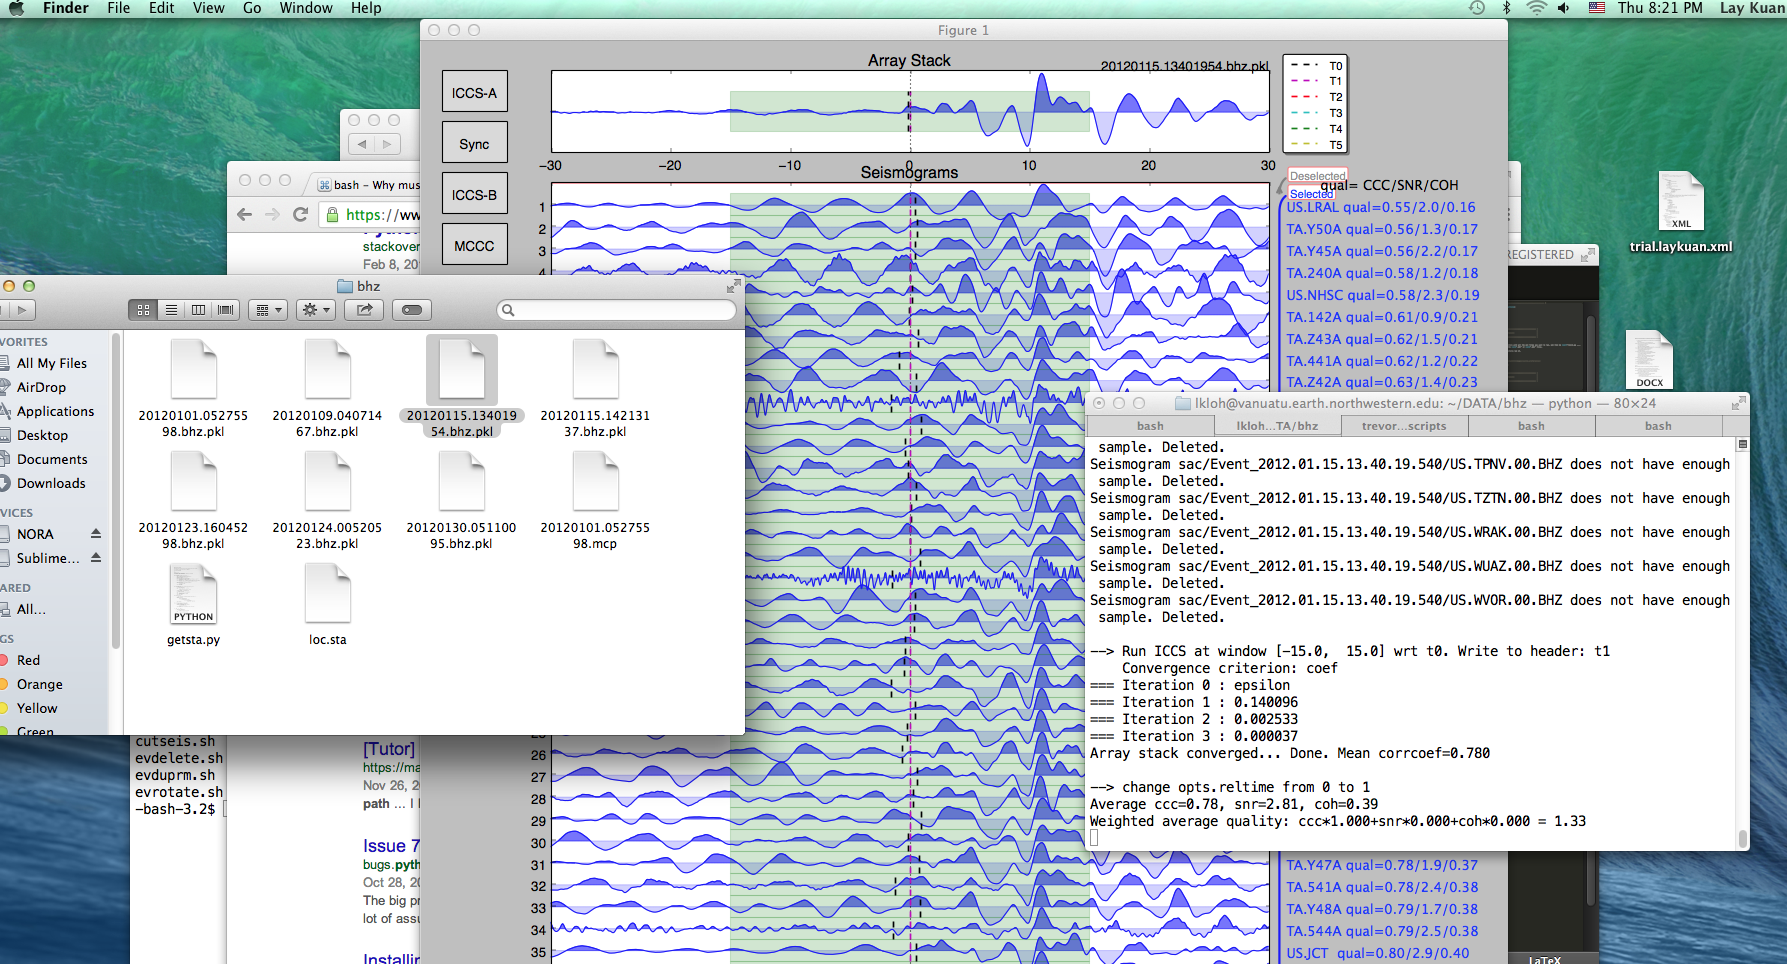
\includegraphics{pick_travel_times.png}


\subsection{Align}
\label{docfiles/PickingTravelTimes:align}
\code{Align} is only used in the beginning, if you have altered some of the travel time arrivals of the seismograms by pressing \code{t2}, and want to realign the array stack.


\subsection{Selecting a time window around the arrival of interest}
\label{docfiles/PickingTravelTimes:selecting-a-time-window-around-the-arrival-of-interest}
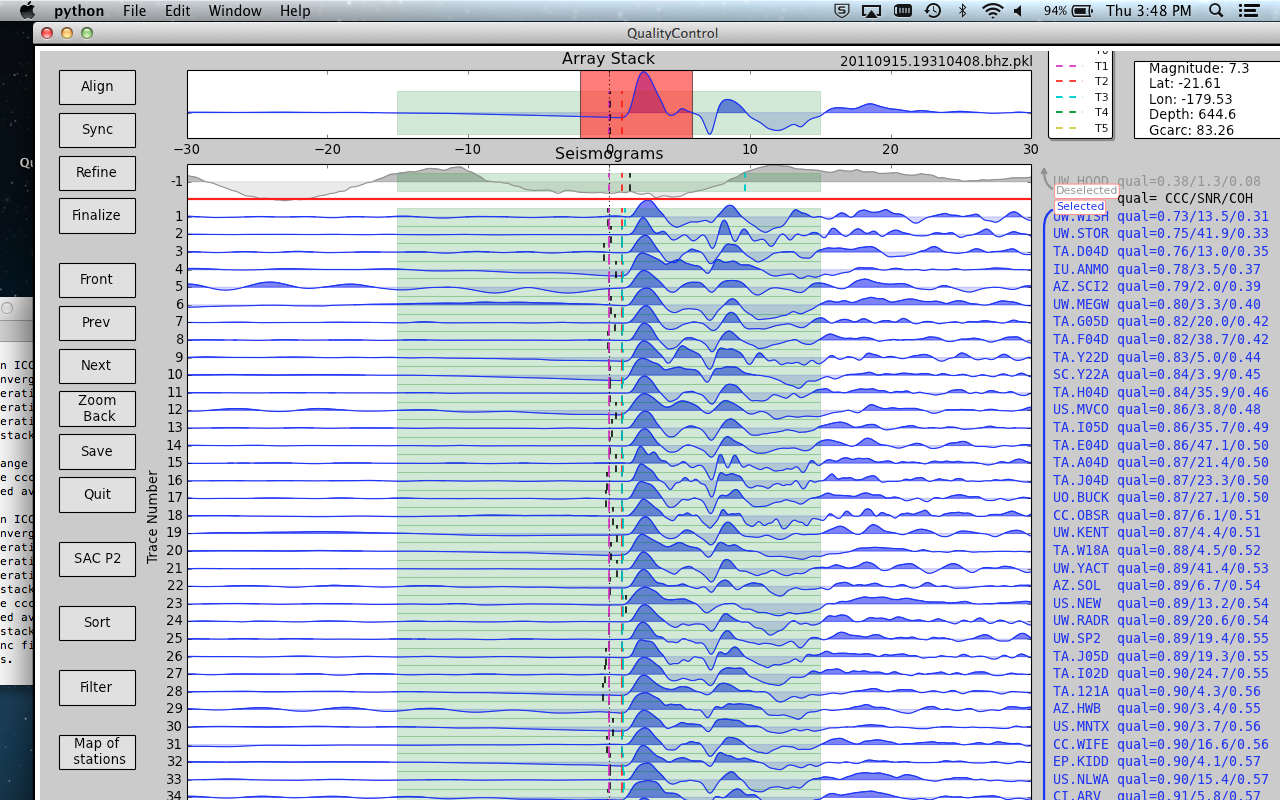
\includegraphics{selecting-time-window-highlight.png}

Hit the \code{Align} button and use \code{t2} to select the arrival time. Now press \code{Sync}. Use the mouse to select the desired time window on the seismogram on the array stack. Press \code{Sync} again.

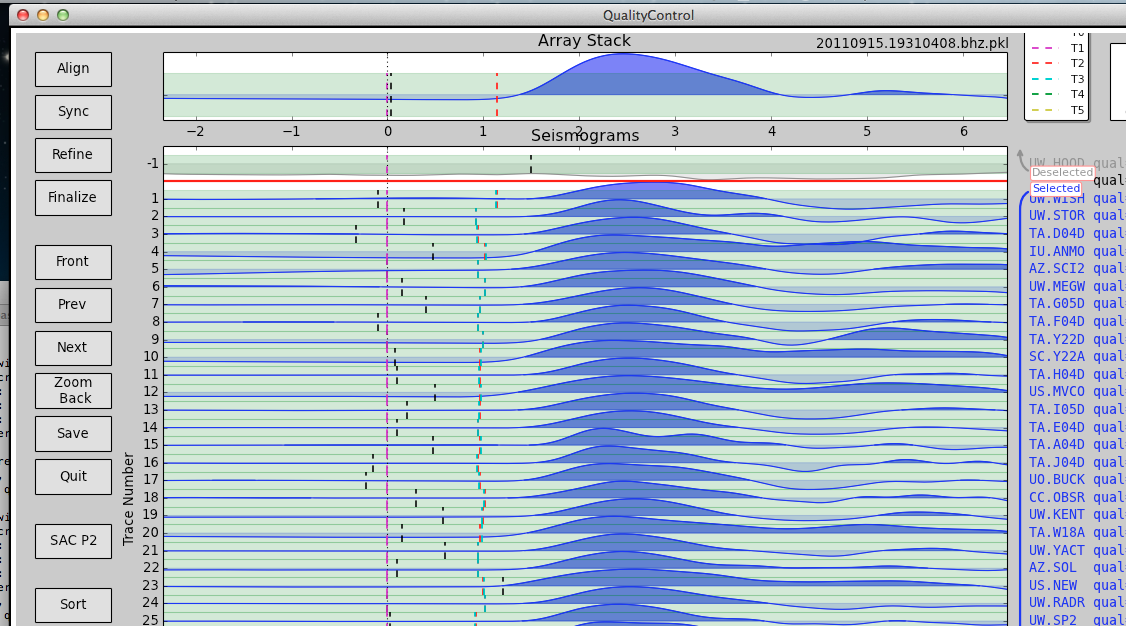
\includegraphics{selected-time-window-t2.png}

Next, set the mouse over the seismogram and press the \emph{w} key. If the new time window has been saved, a message noting the new size of the time window should be printed in the terminal.

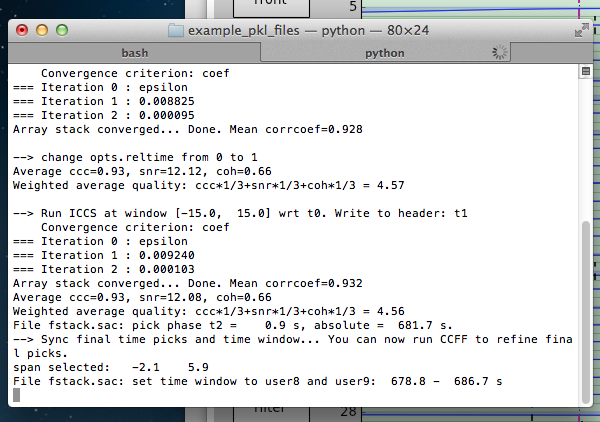
\includegraphics{saved-smaller-time-window.png}

The entire width of the \$x\$-axis is now colored green and will be stored as the time window to use for the cross-correlations. Click the \code{Save Headers Only} button.

Quit the GUI and restart it, and you will see that your new, changed time window is preserved in green in the array stack.

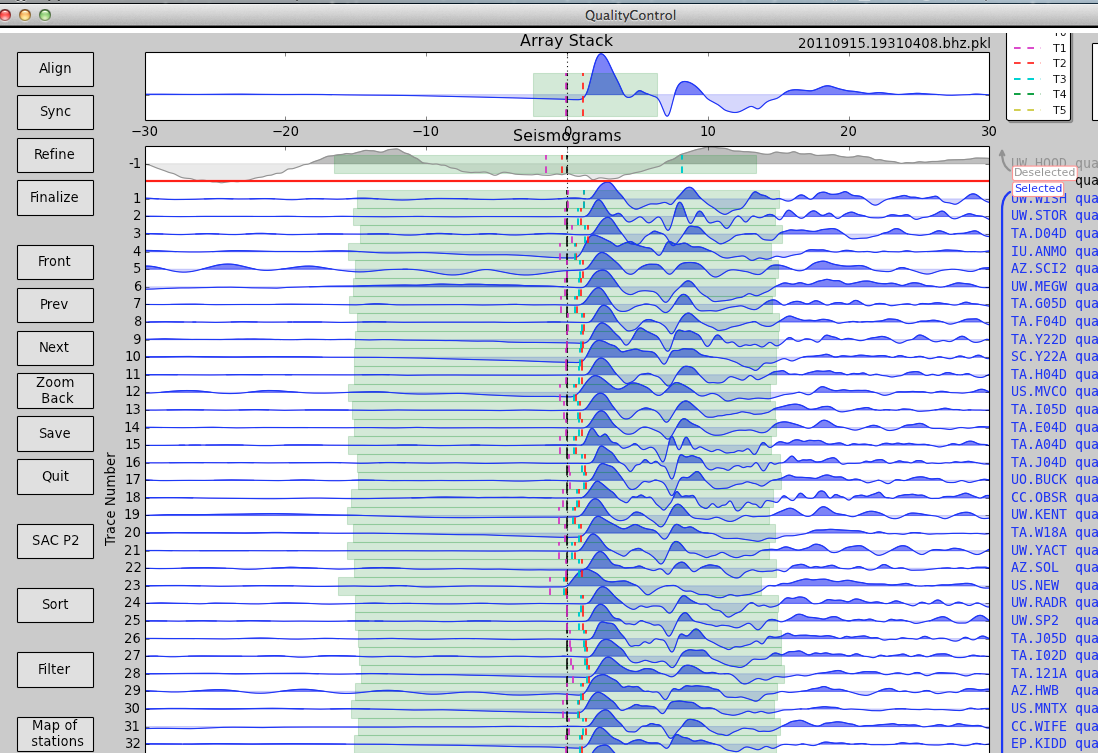
\includegraphics{before-refine-reduced-time-window.png}

Now press \code{refine} and all the seismograms will align with the smaller time window.

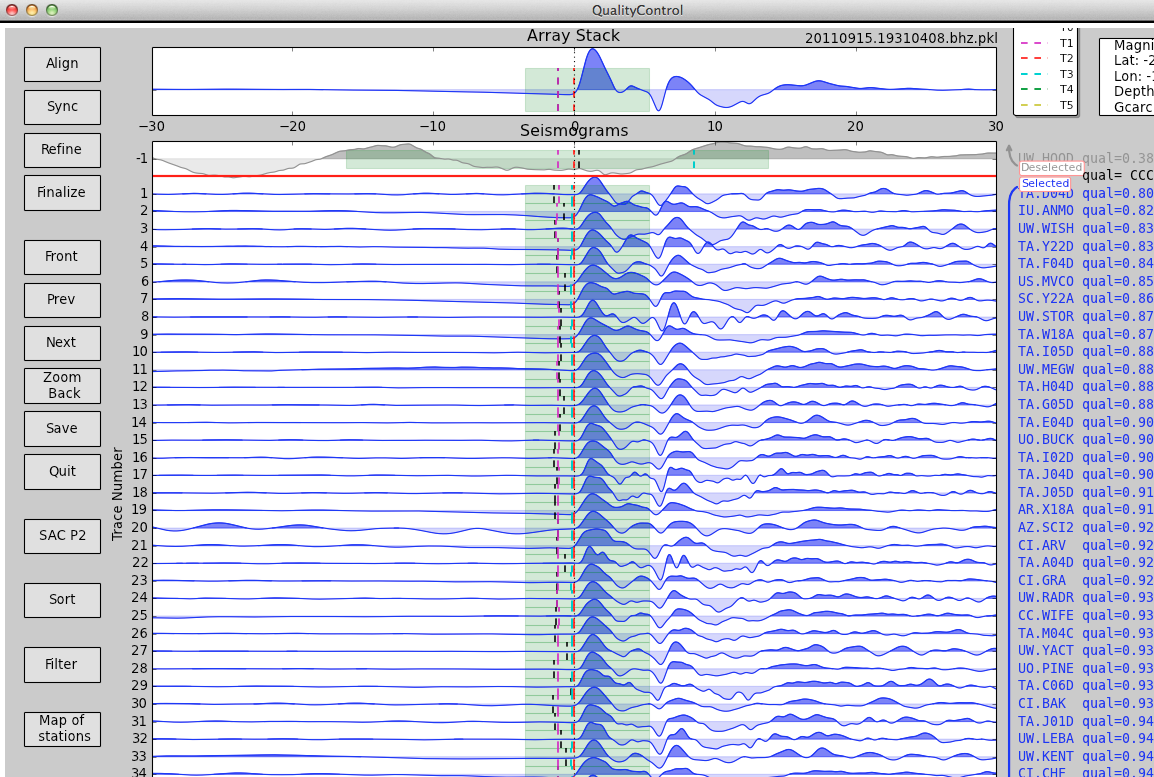
\includegraphics{after-refine-reduced-time-window.png}


\subsection{Get rid of really bad seismograms}
\label{docfiles/PickingTravelTimes:get-rid-of-really-bad-seismograms}
If there are any really bad seismograms, you can click on them to deselect them. Bad seismograms are those that look nothing like the shape of the array stack pictured. Usually, if there are more than enough seismograms, so it is safe to throw out any that deviate more than a bit from the array stack.


\subsection{Filtering}
\label{docfiles/PickingTravelTimes:filtering}
To filter your data, hit the \code{filter} button, and a window will popup for you to use the \href{http://en.wikipedia.org/wiki/Butterworth\_filter}{Butterworth filter} to filter your data.

Remember to save your work periodically once you start picking your travel times, otherwise if AIMBAT crashes, you lose it.

You can choose the order by selecting one of the values provided (default is 1), and choose the low and high frequencies for bandpassing by clicking on the appropriate start and stop frequency on the lower graph.


\subsection{Refine}
\label{docfiles/PickingTravelTimes:refine}
Hit the \code{Refine} button to begin the initial cross-correlations. These appear as red lines.

We are not using \code{Align} here, but these are the theoretical arrival times, marked in black.


\subsection{Finalize}
\label{docfiles/PickingTravelTimes:finalize}
Hit \code{Finalize} to run the Multi-Channel cross-correlation. Do not hit \code{Align} or \code{Refine} again, or all your work will be erased. A warning will pop up to check if you really do want to hit these two buttons if you do click on them.


\subsection{Manually pick the arrival times using t2}
\label{docfiles/PickingTravelTimes:manually-pick-the-arrival-times-using-t2}
For an earthquake, it is expected that the arrival times should be identical in an idealize situation. However, since stations are located in 3D space, this is not necessarily the case. For earthquakes of magnitude 7.0 and above, usually the arrival times are very well aligned as the signal is high. However, if the earthquake is too strong, the source gets complicated, so it needs filtering.

Below a magnitude of 6.0, the signal to noise ratio gets very weak. If the weighted average quality gets too low (1.0 and below), it may not be worth keeping that data set unless you really need it.

We manually pick the the arrival times to align them. Click on the GUI window, hover over the correct spot where you want to pick the new travel time, and type \code{t2}. A red line should appear exactly where your mouse was. You can zoom in to help you with this picking. To zoom out, just hit \code{MCCC} again.

Also pick the arrival time on the array stack. For the arrival times, you want to align the point where the first peak occurs most of all, then try to get the peaks to align.


\subsection{SACP2 to check for outlier seismograms}
\label{docfiles/PickingTravelTimes:sacp2-to-check-for-outlier-seismograms}
Hit and go to the last figure, (d). Zoom in to have a better look. Zooming in doesn’t always work well; close and reopen the \code{SACP2} window if there are problems.

Click on the outliers that stray from the main group of stacked seismograms. The terminal will output the names of the seismograms that you clicked on, so you can return to the main GUI window and readjust the travel times.


\subsection{Go through the badly aligned seismograms and realign the travel times manually}
\label{docfiles/PickingTravelTimes:go-through-the-badly-aligned-seismograms-and-realign-the-travel-times-manually}
By default, the worst seismograms are on the first page, and as you click through the pages, the quality of the seismograms gradually gets better. Keep using \code{t2} to realign the arrival times so that the peaks of all the seismograms are nicely aligned. Remember to zoom in to have a better look.

However, you may which to sort the seismograms in alphabetical order so that you can find the bad seismogrrams and correct them more easily. Hit the \code{sort} button and a window will popup for you to choose which sorting method to use. In this case, choose to sort the files by filename.

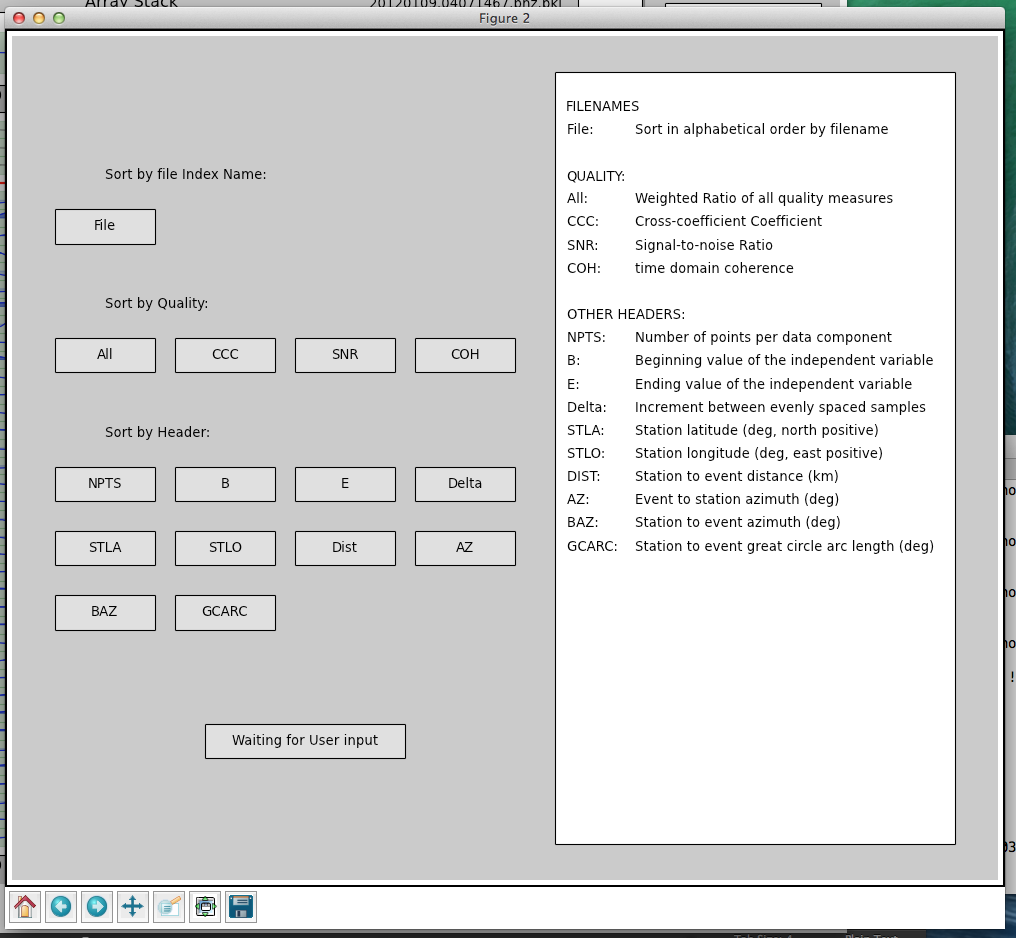
\includegraphics{sorting-interface.png}

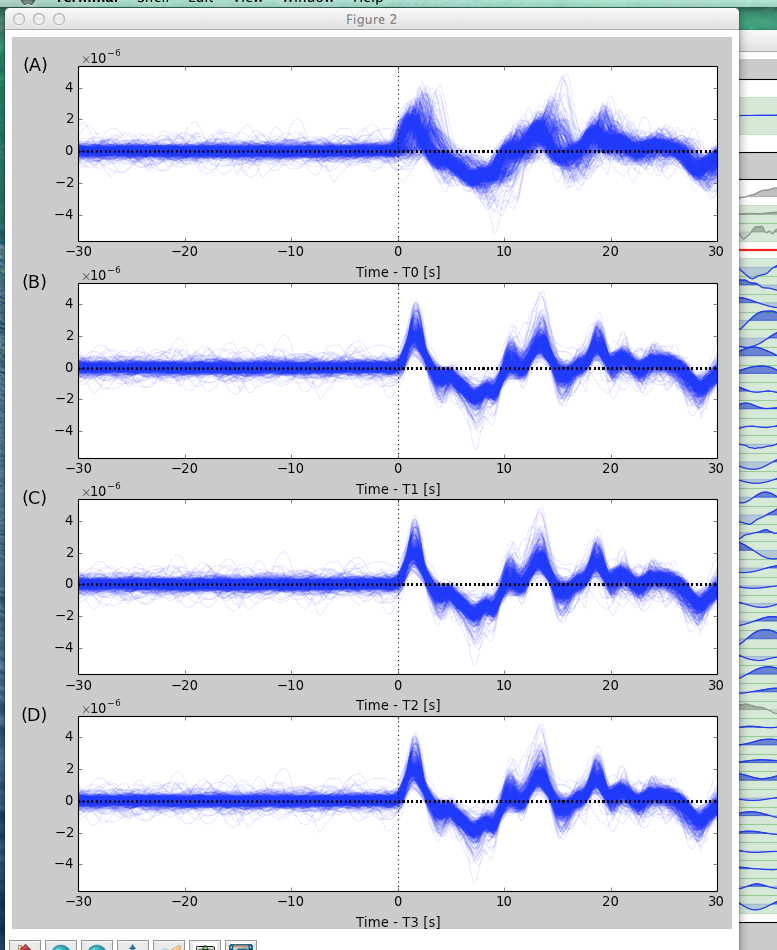
\includegraphics{SACP2_popup.png}

The seismograms are stretched to fit together, but they may be scaled differently.


\section{What the Alignments Stand For}
\label{docfiles/PickingTravelTimes:what-the-alignments-stand-for}\begin{itemize}
\item {} 
T0: Theoretical Arrival

\item {} 
T1: Pick from initial cross correlation

\item {} 
T2: Travel Time pick

\item {} 
T3: MCCC pick

\item {} 
T4: Zoom in

\end{itemize}


\section{Post Processing}
\label{docfiles/PickingTravelTimes:post-processing}

\subsection{Getting the output}
\label{docfiles/PickingTravelTimes:getting-the-output}
In the same folder as the initial PKL file you ran \code{ttpick.py} on, you can find the output list with extension \code{\textless{}event name\textgreater{}.mcp}, which contains the travel time arrivals.

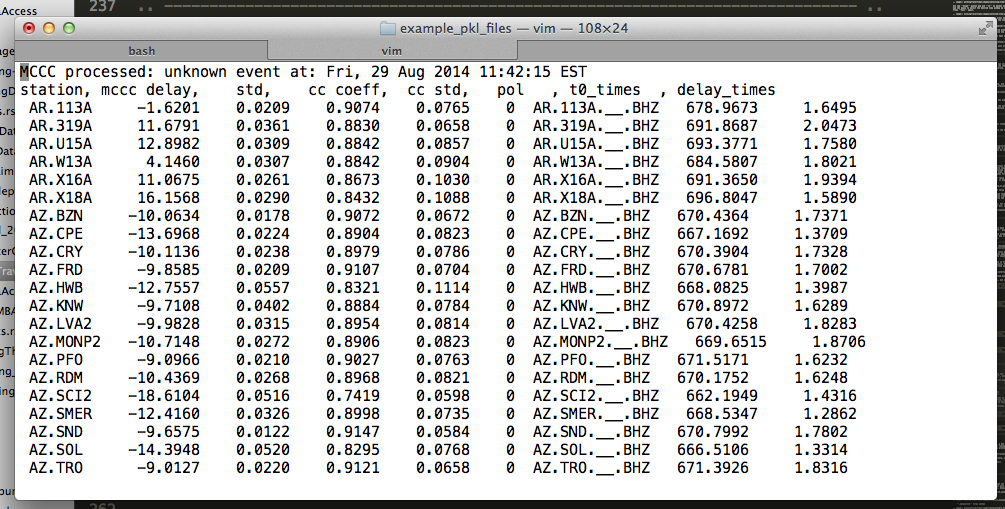
\includegraphics{output_list.png}

\emph{mccc delay{}`} is \emph{t3{}`+average arrival times, and {}`t0\_times} are the theoretical arrival times. \emph{delay\_times} are obtained by taking \$t3-t0\$.


\subsection{Disclaimer about delay times}
\label{docfiles/PickingTravelTimes:disclaimer-about-delay-times}
\emph{t0} depends on hypocenter location, origin time and reference model. We compute the delay time by finding \emph{t3-t0}, but it does not have elliptic, topological, or crust corrections.


\subsection{Getting the stations of the seismograms chosen}
\label{docfiles/PickingTravelTimes:getting-the-stations-of-the-seismograms-chosen}
Run \code{getsta.py} in the additional scripts (not on Github for now). It gives the unique list of stations where the seismograms came from. You need to run it with the list of all \code{pkl} files chosen after you saved to. You so this \code{./getsta.py *.pkl}.

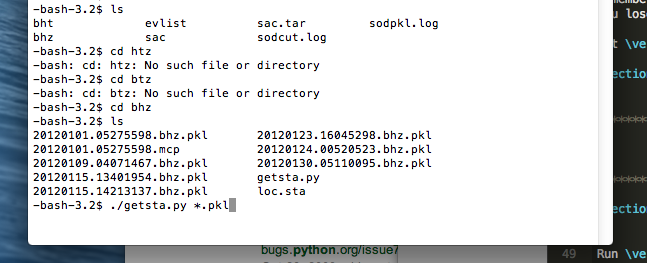
\includegraphics{count_stations.png}


\subsection{Picking Travel Times does not work}
\label{docfiles/PickingTravelTimes:picking-travel-times-does-not-work}
If you run \code{ttick.py \textless{}Event name\textgreater{}.bhz.pkl}, a GUI will pop up for you to manually pick the travel times by pressing the keyboard. If typing on the keyboard as directed does not allow you to pick travel times, it could be a problem with the keyboard settings, or the matplotlib backend.

To fix this, first look for the .matplotlib directory. It is hidden so in your home directory do \code{ls -a} to find it.
Once you have found the \code{.matplotlib} directory, cd into it, and then look for the \code{matplotlibrc} file.
Inside that file, ensure the backend is set to:

\begin{Verbatim}[commandchars=\\\{\}]
backend : TkAgg
\end{Verbatim}

Comment out the other backends!


\subsection{Travel Times}
\label{docfiles/PickingTravelTimes:travel-times}
If one of the seismograms being picked does not fit completely within the green (computer) window, nad you hit \emph{ICCC-A} or \emph{ICCC-B}, you will get an error message complaining about the exact seismogram which is too short. Deselect it.


\chapter{Visualizing Stations on a map}
\label{docfiles/VisualizingStations:visualizing-stations-on-a-map}\label{docfiles/VisualizingStations::doc}
Note: NOT available in \emph{aimbat-stable}.

After running:

\begin{Verbatim}[commandchars=\\\{\}]
ttpick.py \PYGZlt{}sac\PYGZhy{}files\PYGZgt{}
\end{Verbatim}

Red dots represent circles used for computing delay times; black triangles represent discarded stations. Click on a dot to get the station name.

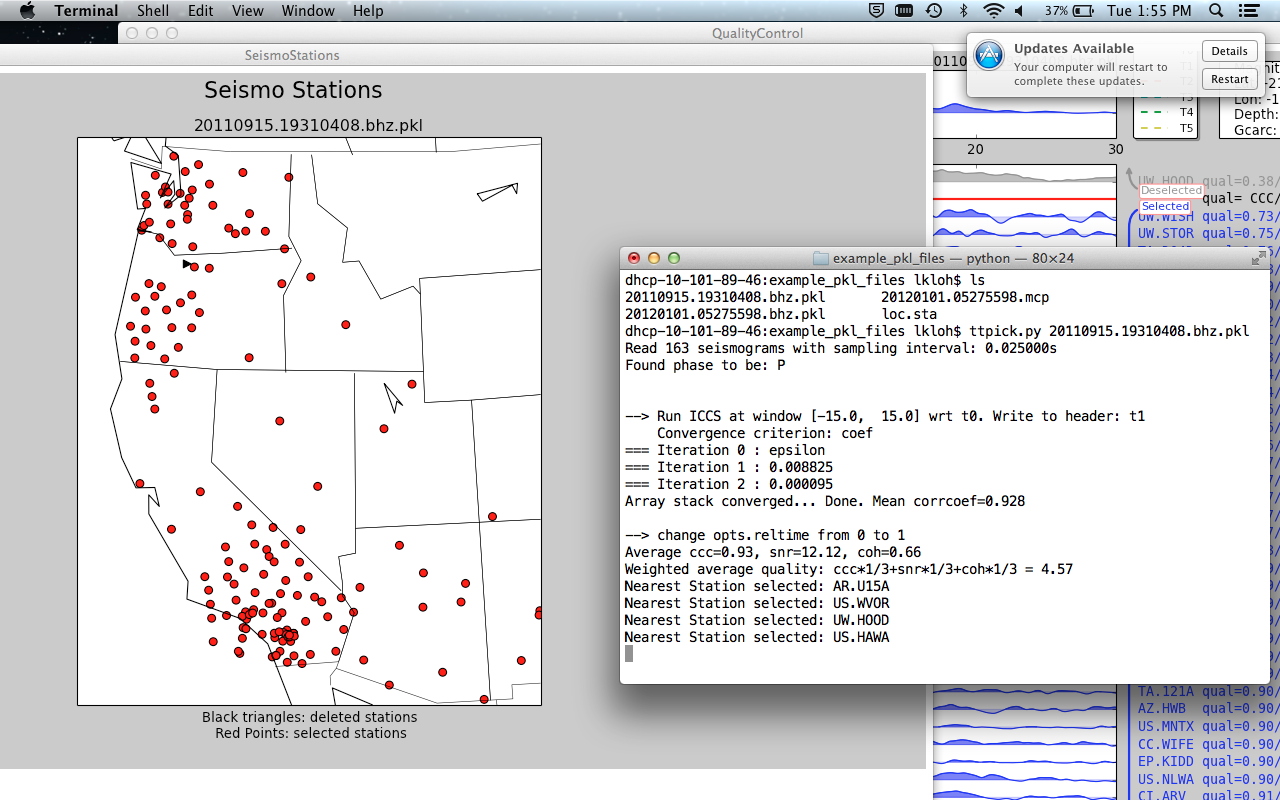
\includegraphics{basemap_stations.png}


\chapter{Unit Testing}
\label{docfiles/unitTests:unit-testing}\label{docfiles/unitTests::doc}
Note: NOT available in \emph{aimbat-stable}.

This section is mainly for those who which to make tweaks to AIMBAT themselves. We have added some unit tests to AIMBAT to ensure its robustness. See the \href{https://docs.python.org/2/library/unittest.html}{Python Unit Testing Framework} for more details.


\section{Running the Tests}
\label{docfiles/unitTests:running-the-tests}
In the AIMBAT repository, \code{cd} into \code{/src/pysmo/unit\_tests} and run:

\begin{Verbatim}[commandchars=\\\{\}]
python run\PYGZus{}unit\PYGZus{}tests.py
\end{Verbatim}


\chapter{Updating this manual}
\label{docfiles/updatingThisManual:updating-this-manual}\label{docfiles/updatingThisManual::doc}
This is for someone who wants to be a collaborator on AIMBAT only. This is NOT necessary for anyone who only wants to use AIMBAT. AIMBAT will work fine if you do not install the dependencies listed here.

To be able to update the manual, download the \href{https://github.com/pysmo/aimbat-docs}{source code} from Github, and install the dependencies.


\section{Dependencies}
\label{docfiles/updatingThisManual:dependencies}\begin{itemize}
\item {} 
\href{http://sphinx-doc.org/}{Sphinx}. Download and install from \href{https://pypi.python.org/pypi/Sphinx}{here}. Don't get the Python Wheel version unless you know what you are doing

\item {} 
\emph{LaTeX}. Download it from \href{http://www.tug.org/mactex/}{here}. Get the package installer.

\item {} 
A browser. But if you are reading this, you already have it.

\end{itemize}


\section{How to update this manual}
\label{docfiles/updatingThisManual:how-to-update-this-manual}
On the master branch, cd into the github repository \emph{aimbat-docs \textless{}https://github.com/pysmo/aimbat-docs\textgreater{}} and run:

\begin{Verbatim}[commandchars=\\\{\}]
sphinx\PYGZhy{}build \PYGZhy{}b html . builddir
make html
make latexpdf
\end{Verbatim}

The two commands builds the html for the webpage, while the last command makes a pdf version of the online documentation.

Now, commit the changes make in github, and push the changes to the master branch. The changes should be visible in the documentation within a few minutes.


\chapter{Citations}
\label{docfiles/citations:citations}\label{docfiles/citations::doc}

\chapter{Indices and tables}
\label{index:indices-and-tables}\begin{itemize}
\item {} 
\emph{genindex}

\item {} 
\emph{modindex}

\item {} 
\emph{search}

\end{itemize}

\begin{thebibliography}{VanDecarCrosson1990}
\bibitem[GoldsteinDodge2003]{GoldsteinDodge2003}{\phantomsection\label{docfiles/citations:goldsteindodge2003} 
Goldstein, P., D. Dodge, M. Firpo, and L. Minner (2003), SAC2000: Signal processing and analysis tools for seismologists and engineers, International Geophysics, 81, 1613–1614.
}
\bibitem[Hunder2007]{Hunder2007}{\phantomsection\label{docfiles/citations:hunder2007} 
Hunter, J. (2007), Matplotlib: A 2D Graphics Environment, Computing in Science \& Engineering, 3(9), 90–95.
}
\bibitem[LouVanDerLee2013]{LouVanDerLee2013}{\phantomsection\label{docfiles/citations:louvanderlee2013} 
AIMBAT: A Python/Matplotlib Tool for Measuring Teleseismic Arrival Times. Xiaoting Lou, Suzan van der Lee, and Simon Lloyd (2013), Seismol. Res. Lett., 84(1), 85-93, doi:10.1785/0220120033.
}
\bibitem[VanDecarCrosson1990]{VanDecarCrosson1990}{\phantomsection\label{docfiles/citations:vandecarcrosson1990} 
VanDecar, J. C., and R. S. Crosson (1990), Determination of teleseismic relative phase arrival times using multi-channel cross-correlation and least squares, Bulletin of the Seismological Society of America, 80(1), 150–169.
}
\bibitem[BulandChapMan1983]{BulandChapMan1983}{\phantomsection\label{docfiles/citations:bulandchapman1983} 
Ray Buland and C. H. Chapman (1983), The Computation of Seismic Travel Times, Bulletin of the Seismological Society of America, 73(5), 1271-1302.
}
\end{thebibliography}



\renewcommand{\indexname}{Index}
\printindex
\end{document}
